\section{Populations} 
\label{sec:population}

\subsection{Systèmes à un spin}
\label{sec:popun}
Un ensemble de $P$ spins isolés en état d'équilibre dans le champ $\bzerovec$
est décrit par la matrice densité initiale
\begin{equation}
\sigma_0 = P \cdot E/2 + \Delta P \cdot I_z
\end{equation}
où 
\begin{equation}
P = p_{\al} + p_{\be} \qetq \Delta P = p_{\al} - p_{\be}
\end{equation}
en faisant intervenir
les populations associées aux niveaux énergétiques $E_{\al}$ et $E_{\be}$.
Ces populations sont aisément déductibles à partir des coefficients
de $E/2$ (qui est toujours égale à $P$) et de $I_z$ :
\begin{equation}
p_{\al} = \frac{P + \Delta P}{2} \qetq p_{\be} = \frac{P + \Delta P}{2}
\end{equation}

D'une manière générale, si
\begin{equation}
\sigma = a \cdot E/2 + b \cdot I_x + c \cdot I_y + d \cdot I_z
\end{equation}
alors
\begin{equation}
p_{\al} = \frac{a+d}{2} \qetq p_{\be} = \frac{a-d}{2}
\end{equation}
ce qui impose à $a$ et $d$ d'être des nombres réels.

L'invariance de $E/2$ et de $I_z$ sous l'action de l'opérateur
d'évolution libre entraîne l'invariance les populations des
états énergétiques pendant ces périodes, en l'absence de relaxation
longitudinale.

Une impulsion d'angle $\theta$ et de phase quelconque
exercée sur un système en équilibre transforme $I_z$ en
$\cos\theta \cdot I_z + ...$ et conduit donc à
\begin{equation}
p_{\al} = P\frac{1+\cos\theta}{2} \qetq
p_{\be} = P\frac{1-\cos\theta}{2}
\end{equation}
avec pour conséquence que si $\theta = \pi / 2$, alors les populations
sont égales et la composante longitudinale de l'aimantation est nulle
(certains auteurs parlent alors de saturation, même si l'aimantation
transversale est non nulle).
Une impulsion d'angle de nutation $\pi$ échange $p_{\al}$ et $p_{\be}$,
conduisant à ce qui est désigné par "inversion de population".
Le retour à l'équilibre est alors uniquement assuré par
la relaxation longitudinale (en négligeant le "radiation damping"...).
L'inversion de population offre donc un moyen, parmi d'autres, de mesurer
le temps de relaxation $T_1$ d'un système.

Notons qu'il est aussi possible d'écrire
\begin{equation}
\sigma = \frac{a+d}{2} \cdot \frac{E + 2I_z}{2} + \frac{a-d}{2} \cdot \frac{E - 2I_z}{2}
+ b \cdot I_x + c \cdot I_y
\end{equation}
qui, en introduisant les matrices
\begin{equation}
I_{\al} = \frac{E + 2I_z}{2} \qetq I_{\be} = \frac{E - 2I_z}{2}
\end{equation}
se transforme en
\begin{equation}
\sigma = p_{\al} \cdot I_{\al} + p_{\be} \cdot I_{\be} + b \cdot I_x + c \cdot I_y
\end{equation}

Le choix de $I_{\al}$ et $I_{\be}$ comme matrices de base au lieu de $E/2$ et $I_z$
donne directement accès aux populations des différents états énergétiques
possibles pour les noyaux.
Ces opérateurs sont pour cette raison appelés opérateurs de population.
L'écriture de $\sigma$ sous la forme:
\begin{equation}
\sigma = p_{\al} \cdot I_{\al} + p_{\be} \cdot I_{\be} 
+ \frac{b-ic}{2} \cdot I_+ + \frac{b+ic}{2} \cdot I_-
\end{equation}
présente la matrice densité comme combinaison linéaire des opérateurs
de population et des cohérences, représentation qui est la
plus "naturelle" (un mathématicien dirait "canonique")
d'après la définition de la matrice densité d'un système.
Toutefois, la simplicité des règles de calcul est en faveur de l'emploi de la
base des opérateurs cartésiens pour l'étude de l'évolution de $\sigma$
sous l'action des hamiltoniens usuels (évolution libre et impulsions de
radio-fréquence).

\subsection{Systèmes à deux spins}

Dans les systèmes à deux spins $IS$, quatre populations 
$p_{\al\al}$, $p_{\al\be}$, $p_{\be\al}$ et $p_{\be\be}$ sont à 
considérer, correspondant chacune à un état $m_s = \pm 1/2$ pour chaque noyau du système.  
Dans un cas général, la matrice densité contient l'information relative aux populations par 
l'intermédiaire des termes proportionnels à $E/2$, $I_z$, $S_z$ et $2I_zS_z$.
Si l'état du système est décrit par
\begin{equation}
\sigma = a_{E/2} \cdot E/2 + a_{I_z} \cdot I_z + a_{S_z} \cdot S_z + 
a_{2I_zS_z} \cdot 2I_zS_z + \mbox{autres termes...}
\end{equation}
alors
\begin{eqnarray}
2a_{E/2} & = & p_{\al\al} + p_{\al\be} + p_{\be\al} + p_{\be\be} = P \\
2a_{I_z} & = & p_{\al\al} + p_{\al\be} - p_{\be\al} - p_{\be\be} = \Delta P(I) \\
2a_{S_z} & = & p_{\al\al} - p_{\al\be} + p_{\be\al} - p_{\be\be} = \Delta P(S) \\
2a_{2I_zS_z} & = & p_{\al\al} - p_{\al\be} - p_{\be\al} + p_{\be\be} 
\end{eqnarray}
ce qui montre que l'état initial du système est décrit par
\begin{equation}
\sigma_0 = P/2 \cdot {E/2} + \Delta P(I)/2 \cdot I_z + \Delta P(S)/2 \cdot S_z
\end{equation}
$P$ (comme $\Delta P(I)$ et $\Delta P(S)$) intervient ici avec un facteur 2 au dénominateur.
Cela se justifie de manière suivante : si toutes les populations sont égales, la
population de chaque état énergétique est $P/4$.
Dans ce cas $\sigma = P/4 \cdot E$ et donc les termes diagonaux de la matrice densité
sont égaux aux populations.
Dans la mesure où la matrice densité n'a pas été définie, cette explication relève
plutôt du moyen mnémotechnique mais n'est pas sans fondement théorique.

Le terme proportionnel à $2I_zS_z$ apparaît dans les systèmes hors équilibre,
même dépourvus d'aimantation transversale.
Son rôle sera détaillé dans l'étude du transfert d'aimantation.

Les populations se déduisent des coefficients multiplicatifs des opérateurs cartésiens 
à l'aide des relations :
\begin{eqnarray}
\label{eqn:popisa}
2 p_{\al\al} & = & a_{E/2} + a_{I_z} + a_{S_z} + a_{2I_zS_z} \\
2 p_{\al\be} & = & a_{E/2} + a_{I_z} - a_{S_z} - a_{2I_zS_z} \\
2 p_{\be\al} & = & a_{E/2} - a_{I_z} + a_{S_z} - a_{2I_zS_z} \\
\label{eqn:popisd}
2 p_{\be\be} & = & a_{E/2} - a_{I_z} - a_{S_z} + a_{2I_zS_z}
\end{eqnarray}
Alternativement, $\sigma$ s'écrit comme combinaison des quatre opérateurs de population :
\begin{equation}
\sigma = p_{\al\al} \cdot P_{\al\al} + p_{\al\be} \cdot P_{\al\be}
+ p_{\be\al} \cdot P_{\be\al} + p_{\be\be} \cdot P_{\be\be} + \mbox{autres termes...}
\end{equation}
avec
\begin{eqnarray}
2 P_{\al\al} = E/2 + I_z + S_z + 2I_zS_z \\
2 P_{\al\be} = E/2 + I_z - S_z - 2I_zS_z \\
2 P_{\be\al} = E/2 - I_z + S_z - 2I_zS_z \\
2 P_{\be\be} = E/2 - I_z - S_z + 2I_zS_z
\end{eqnarray}

Comme pour les systèmes à un spin, les populations n'évoluent pas sous l'action des 
opérateurs de déplacement chimique. 
Elles n'évoluent pas non plus sous l'action de 
l'opérateur de couplage.

Une connaissance un peu plus approfondie de la théorie de la matrice densité
laisse apparaître qu'un opérateur de population $P_{ij}$ de l'ensemble
des états d'un système à deux spins est en fait le produit (direct) des
opérateurs $I_{i}$ et $S_{j}$ ($i$ et $j$ valant $\al$ ou $\be$).
La base des 16 produits des opérateurs cartésiens obtenue à partir des
bases \{$E_I/2$, $I_x$, $I_y$, $I_z$\} et \{$E_S/2$, $S_x$, $S_y$, $S_z$\} peut être
remplacée par celle des produits formés à partir des bases
\{$I_{\al}$, $I_{\be}$, $I_+$, $I_-$\} et 
\{$S_{\al}$, $S_{\be}$, $S_+$, $S_-$\}.
Cette base produit contient
\begin{enumerate}
\item 4 opérateurs de population : 
$I_{\al}S_{\al}$, $I_{\al}S_{\be}$, $I_{\be}S_{\al}$, $I_{\be}S_{\be}$
\item 4 cohérences à simple quanta de $I$ : 
$I_+S_{\al}$, $I_+S_{\be}$, $I_-S_{\al}$, $I_-S_{\be}$
\item 4 cohérences à simple quanta de $S$ : 
$I_{\al}S_+$, $I_{\be}S_+$, $I_{\al}S_-$, $I_{\be}S_-$
\item 2 cohérences à double quanta : $I_+S_+$, $I_-S_-$
\item 2 cohérences à zéro quanta : $I_+S_-$, $I_-S_+$
\end{enumerate}

Comme pour un spin isolé, cette base est idéale tant que le système est soumis
à des périodes d'évolution libre contenant tous les termes de
l'hamiltonien correspondant.
Il est toutefois souvent utile de faire agir séparément les différentes
parties de l'hamiltonien, ainsi que, bien entendu des impulsions de radiofréquence.
La base des produits des opérateurs cartésiens reste alors un bon compromis
pour la facilité de conduite des calculs.
Les règles de prévision de l'évolution de la matrice densité exprimées dans la
base \{$E_I/2$, $I_+$, $I_-$, $I_z$\} et les produits d'opérateurs qui en dérivent
sont parfois très commodes pour analyser certaines situations.
Les règles de calcul correspondantes seront introduites ou rappelées en temps utile.

\subsection{Systèmes à trois spins}

La généralisation des équations régissant les populations à des systèmes à trois spins,
bien que fastidieuse, se fait sans plus de difficulté que pour les systèmes à deux spins.
Ainsi, avec les mêmes notations que ci-dessus :
\begin{equation}
\sigma_0 = P/4 \cdot E/2 + \Delta P(I)/4 \cdot I_z + 
\Delta P(S)/4 \cdot S_z + \Delta P(L)/4 \cdot L_z
\end{equation}
Le facteur 4 devient 8 pour les systèmes à quatre spins, 
et est multiplié par 2 chaque fois qu'il y a un noyau de plus dans le système de spins.

Le coefficient $a_{4I_zS_zL_z}$ de l'opérateur d'ordre longitudinal $4I_zS_zL_z$
se déduit des populations par :
\begin{eqnarray}
4a_{4I_zS_zL_z} & = & p_{\al\al\al} - p_{\al\al\be} - p_{\al\be\al} + p_{\al\be\be}
\nonumber\\
& & \quad - p_{\be\al\al} + p_{\be\al\be} + p_{\be\be\al} - p_{\be\be\be}
\end{eqnarray}

Les relations qui donnent les différentes populations en fonction des coefficients
multiplicatifs des opérateurs cartésien s'écrivent, par exemple, 
\begin{eqnarray}
2p_{\al\al\al} & = & a_{E/2} + a_{I_z} + a_{S_z} + a_{L_z}
\nonumber\\
& & \quad + a_{2I_zS_z} + a_{2I_zL_z} + a_{2S_zL_z} + a_{4I_zS_zL_z}
\end{eqnarray}
le facteur 2 restant à l'identique quel que soit le nombre de spins dans le système.
L'opérateur de population $P_{\al\al\al}$ dont le facteur multiplicatif est 
la population $p_{\al\al\al}$ est alors donné par :
\begin{eqnarray}
4P_{\al\al\al} & = & E/2 + I_z + S_z + L_z
\nonumber\\
& & + 2I_zS_z + 2I_zL_z + 2S_zL_z + 4I_zS_zL_z
\end{eqnarray}

\section{Echo de spin}
\label{sec:echodespin}

De nombreuses séquences d'impulsions contiennent le motif $T$ -- ($\pi$) -- $T$, 
considéré comme un délai d'évolution de durée $2T$ "coupé" en son milieu par une impulsion 
RF d'angle $\pi$
comme indiqué par la figure \ref{fig:echo}.

\begin{figure}[hbt]
\setlength{\unitlength}{5mm}
\begin{center}
\begin{picture}(16,6)
\put(0,1){\vector(1,0){16}}
\put(2,4){\vector(0,-1){3}}
\put(2,4.5){\makebox(0,0){$\sigma_0$}}
\put(6.7,4){\vector(1,-3){1}}
\put(6.8,4.5){\makebox(0,0){$\sigma_1$}}
\put(9.2,4){\vector(-1,-3){1}}
\put(9.3,4.5){\makebox(0,0){$\sigma_2$}}
\put(14,4){\vector(0,-1){3}}
\put(14,4.5){\makebox(0,0){$\sigma_3$}}
\put(5,3){\makebox(0,0){$T$}}
\linethickness{2mm}
\put(7.95,1){\line(0,1){3}}
\thinlines
\put(11,3){\makebox(0,0){$T$}}
\put(16,2){\makebox(0,0){$t$}}
\put(8,5){\makebox(0,0){$\pi_{\phi}$}}
\end{picture}
\end{center}
\caption{\label{fig:echo}
Echo de spin
}
\end{figure}

Les modifications subies par la matrice densité d'un système entre l'instant initial 
et l'instant final de cette séquence sont calculables par les règles usuelles 
de transformation des matrices de base. 
Il est néanmoins possible de simplifier les calculs en 
appliquant successivement l'impulsion RF et un 
opérateur d'évolution appelé opérateur réduit.
Leur action est identique à celle effectuée par la 
succession des opérateurs associés à la séquence considérée. 
L'opérateur associé à une évolution libre de durée $2T$ est en fait amputé 
de certains termes suivant la nature du 
système de spins considéré et la sélectivité de l'impulsion d'angle $\pi$.
L'impulsion centrale est associée à l'opérateur noté $O_{\pi}$.

Un traitement général de ce problème nécessiterait à nouveau de recourir à la
théorie générale de l'opérateur densité. 
Seuls les résultats seront donnés ici, avec tout de même une justification
satisfaisante pour l'esprit.
Le lecteur pourra à volonté vérifier que la transformation d'une matrice de base 
quelconque par la suite "normale" d'opérateurs (évolution libre, impulsion RF puis
évolution libre) et par le raccourci de l'opérateur réduit coïncident :
\begin{equation}
\flham{T \cdot H} \quad 
\flham{O_{\pi}} \quad
\flham{T \cdot H}
\iff
\flham{O_{\pi}} \quad
\flham{2T \cdot \hred}
\end{equation}
Une autre manière de se persuader de l'exactitude du résultat sur des cas particuliers
est de considérer l'évolution du vecteur aimantation dans le cadre du modèle
de Bloch et de son extension aux systèmes couplés.

\subsection{Système à un spin}
\label{sec:echo1spin}
Si le système étudié est constitué d'un unique noyau $I$,
la règle qui donne l'expression de l'opérateur réduit s'établit aisément.

Pour avoir une vue globale de l'action de la séquence d'écho de spin, il faut
commencer par savoir comment sont transformées les matrices de base $I_x$, $I_y$ et $I_z$.

La matrice de base $\sigma_0 = I_z$ est invariante pendant la première période d'évolution, se 
transforme en $\sigma_2 = -I_z$ ($\cos\pi = -1$, $\sin\pi = 0$) 
sous l'action de l'impulsion d'angle $\pi$, quelque soit sa phase, 
reste ensuite égale à $-I_z$ jusqu'à la fin de la séquence ($\sigma_3 = -I_z$).

Considérons maintenant l'évolution de $\sigma_0 = I_x = (I_+ + I_-)/2$. 
Entre les instants 0 et 1, $I_+$ évolue en $\exp(-i\omsi T) \cdot I_+$
et $I_-$ en $\exp(+i\omsi T) \cdot I_-$.
Juste avant l'impulsion, la matrice densité du système est 
donc :
\begin{equation}
\sigma_1 = (\exp(-i\omsi T) \cdot I_+ + \exp(+i\omsi T) \cdot I_-)/2
\end{equation}
Sachant que 
\begin{eqnarray}
I_x & \flham{\pi I_x} & I_x \\
I_y & \flham{\pi I_x} & -I_y \\
I_x & \flham{\pi I_y} & -I_x \\
I_y & \flham{\pi I_y} & I_y
\end{eqnarray}
on détermine que
\begin{eqnarray}
I_+ = I_x + iI_y \flham{\pi I_x} I_x - iIy = I_- \\
I_- = I_x - iI_y \flham{\pi I_x} I_x + iIy = I_+ \\
I_+ = I_x + iI_y \flham{\pi I_y} -I_x + iIy = -I_- \\
I_- = I_x - iI_y \flham{\pi I_y} -I_x - iIy = -I_+
\end{eqnarray}

A l'instant 2, si la phase $\phi$ de l'impulsion est nulle, 
la matrice densité du système vaut :
\begin{equation}
\sigma_2 = (\exp(-i\omsi T) \cdot I_- + \exp(+i\omsi T) \cdot I_+)/2
\end{equation}
Pendant le second délai de durée $T$, $I_+$ et $I_-$ évoluent 
comme pendant le premier délai et donc
\begin{eqnarray}
\sigma_3 & = & (\exp(-i\omsi T)\exp(+i\omsi T) \cdot I_- \nonumber\\
& & \quad + \exp(+i\omsi T)\exp(-i\omsi T) \cdot I_+)/2 \\
& = & (I_- + I_+)/2 \\
& = & I_x
\end{eqnarray}

La transformation subie par $I_x$, $I_y$ et $I_z$ suivant la phase de l'impulsion 
est donnée dans le tableau \ref{tab:echo}.

\begin{table}
\caption{\small Influence de la phase de l'impulsion d'angle $\pi$ sur l'aimantation
issue de l'écho de spin}
\label{tab:echo}
\begin{center}
\begin{tabular}[hbt]{ccc}
                  & $\pi_x$ & $\pi_y$ \\[1.5ex]
$I_x \rightarrow$ & $I_x$   & $-I_x$  \\
$I_y \rightarrow$ & $-I_y$  & $I_y$   \\
$I_z \rightarrow$ & $-I_z$  & $-I_z$
\end{tabular}
\end{center}  
\end{table}

Tout se passe donc comme si toutes les matrices de base ne subissaient que l'action de 
l'impulsion $\pi_{\phi}$, quelque soit sa phase $\phi$.
On constate que l'impulsion a supprimé complètement l'opérateur d'évolution libre 
de durée de $2T$, et que seul l'opérateur 
associé à l'impulsion est à prendre en compte.

Dans le cas du système à un spin, l'opérateur réduit est donc l'opérateur nul (celui
qui donne toujours zéro),
associé au super--opérateur identité (celui qui ne fait rien,
comme il se doit pour un opérateur nul).

Un tel résultat est aisément visualisé à l'aide du modèle vectoriel.
Alternativement, l'évolution de $I_-$ est intéressante à considérer.
A l'instant 1, son coefficient multiplicatif est $\exp(+i\omsi T)$ et devient
brusquement (les impulsions sont idéales et donc infiniment brèves),
à l'instant 2, $\exp(+i\omsi T)$,
qui était le coefficient de $I_+$ à l'instant 1.
Tout s'est passé pendant l'impulsion comme si $T$ était devenu $-T$.
Une impulsion $\pi$ est donc une sorte de machine à remonter (ou à inverser) le temps.
De manière équivalente, il suffit de considérer que l'impulsion a
transformé $\omsi$ en $-\omsi$ pendant la première période d'évolution libre.
Le seconde période de durée $T$ ne fait qu'annuler ce qui s'est passé pendant la première.
Il est donc normal que le résultat ne fasse pas intervenir la valeur de $\omsi$.

Le terme d'écho de spin a pour origine le comportement de l'aimantation
macroscopique en présence d'un champ statique $\bzerovec$ inhomogène.
Au terme du premier délai de durée $T$ différents vecteurs aimantation
liés à différentes localisations spatiales dans l'échantillon ont tourné
autour de $OZ$ avec des angles différents, comme indiqué sur la
figure \ref{fig:isochrom}, page \pageref{fig:isochrom}.
Cela revient à dire que les différentes régions de l'espace
sont associées à diverses valeurs de $\omsi$.
Il se peut très bien que $\aimvec$ soit nul à l'instant 1 pour cause
de déphasage total de ses différentes composantes (aussi appelées \emph{isochromats}).
L'impulsion RF et le second délai vont amener chacune des composantes sur
l'axe $OX$, indépendemment de leur position dans l'échantillon, 
car indépendemment de leur $\omsi$.
L'aimantation totale est ainsi "ressucitée" à l'instant 3, comme un écho
de la situation du système à l'instant 0.

L'impulsion d'angle $\pi$ appliquée à l'aimantation transversale est
appelée impulsion de \emph{refocalisation} puisqu'elle la ramène à son intensité
initiale après avoir été \emph{défocalisée} par les inhomogénéités de $\bzerovec$.
Un affaiblissement de l'aimantation après le temps $2T$ est tout de même présent, 
lié à deux phénomènes physiques. 
Le premier, déjà cité, est la relaxation transversale, que rien ne peut refocaliser.
Le second, qui est aussi irréversible, 
est lié à la diffusion translationnelle des molécules dans le cas
d'échantillons liquides : ce que subit une molécule pendant le premier délai
n'est parfaitement compensé pendant le second que si la molécule est restée à la même place.
Plus les molécules bougent vite et moins la refocalisation des isochromats
sera effective et plus le signal sera atténué.
L'écho de spin est donc la technique expérimentale de base pour accéder à la fois
aux temps $T_2$ "vrais" et à la mobilité des molécules en solution.

Le recours aux opérateurs $I_+$ et $I_-$ n'était pas strictement nécessaire ici.
Il a cependant permis de montrer aussi qu'une impulsion d'angle $\pi$ entraîne
une variation d'ordre de cohérence de $\pm 2$ pour les états d'ordre $\mp 1$,
ce qui ne sera pas sans importance par la suite.
Si l'aimantation initiale est longitudinale, elle le reste, mais change de sens.
On parle alors d'impulsion d'\emph{inversion} (voir paragraphe \ref{sec:popun}).

\subsection{Systèmes à deux spins}

Nous considérons ici un système $IS$ faiblement couplé.

\subsubsection{Principe}
Pour trouver $\hred$, il suffit d'écrire $H$ et de n'en garder que les termes qui sont
invariants par action de $O_{\pi}$.

Il n'y a dans le principe que deux possibilités pour $O_{\pi}$ :
soit la refocalisation ne s'exerce que sur $I$ (ou sur $S$),
soit elle s'exerce sur $I$ et $S$ simultanément.
Dans le premier cas, l'impulsion est dite sélective.
Le second cas, où la refocalisation n'est pas sélective, 
est celui des sytèmes homonucléaires où
$O_{\pi} = \pi \cdot (I_{\phi} + S_{\phi})$ ainsi que celui des
systèmes hétéronucléaires où deux impulsions d'angle $\pi$ sont appliquées
simultanément avec des phases qui ne sont pas nécessairement identiques.

Dans le premier cas, si $O_{\pi} = \pi \cdot I_{x,y}$
L'hamiltonien d'évolution libre
\begin{equation}
H = \omsi \cdot I_z + \omss \cdot S_z + \pi J \cdot 2I_zS_z
\end{equation}
est réduit en
\begin{equation}
\hred = \omss \cdot S_z
\end{equation}
car
\begin{eqnarray}
I_z  & \flham{\pi \cdot I_{x,y}} & -I_z \\
S_z  & \flham{\pi \cdot I_{x,y}} & S_z \\
2I_zS_z  & \flham{\pi \cdot I_{x,y}} & -2I_zS_z
\end{eqnarray}
Il y a alors refocalisation de l'offset de $I$ et du couplage.
Tout se passe en effet comme si $\omsi = J = 0$.
Par symétrie si l'impulsion $\pi$ ne s'applique qu'au noyau $S$,
ce sont son offset et le couplage qui sont refocalisés.

Dans le second cas, $O_{\pi} = \pi \cdot I_{x,y} + \pi \cdot S_{x,y}$.
Sachant que :
\begin{eqnarray}
I_z  & \flham{\pi \cdot I_{x,y}} 
\flham{\pi \cdot S_{x,y}} & -I_z \\
S_z  & \flham{\pi \cdot I_{x,y}} 
\flham{\pi \cdot S_{x,y}} & -S_z \\
2I_zS_z  & \flham{\pi \cdot I_{x,y}} 
\flham{\pi \cdot S_{x,y}} & 2I_zS_z
\end{eqnarray}
et donc que seul le terme de couplage est invariant par action de $O_{\pi}$
\begin{equation}
\label{eqn:hredis}
\hred = \pi J \cdot 2I_zS_z
\end{equation}
Les effets des offsets sont refocalisés et seule l'action du couplage
subsiste.
On voit que l'on dispose ici d'un outil extrêmement puissant
qui permet au spectroscopiste de trier parmi les termes de
l'hamiltonien ceux qui l'intéressent.
Une grande partie de ce qui constitue les chapitres suivants est
basée sur les idées présentées dans ce paragraphe.

\subsubsection{Exemple avec $\pi_x(I)$ seul}
Il n'est pas inintéressant d'étudier un exemple en regardant
ce qui ce passe en utilisant la base des cohérences et des populations,
en partant de $\sigma_0 = I_x$ et avec, dans un premier temps
$O_{\pi} = \pi \cdot I_x$.
Sachant que $I_x = I_xE_S$, $2I_x = I_+ + I_-$ et que $E_S = S_{\al} + S_{\be}$,
\begin{equation}
2\sigma_0 = I_+S_{\al} + I_+S_{\be} + I_-S_{\al} + I_+S_{\be}
\end{equation}
Pour prendre des notations cohérentes avec les définitions de $\nu_1$ et de $\nu_2$
pour le système $IS$, on définit :
\begin{equation}
\Omega_1 = \omsi -\pi J = 2\pi\nu_1 \qetq
\Omega_2 = \omsi +\pi J = 2\pi\nu_2
\end{equation}
ce qui, d'après les équations 
\ref{eqn:evolipmsa-is} et \ref{eqn:evolipmsb-is}
donne après la première période d'évolution libre :
\begin{eqnarray}
2\sigma_1 & = & \exp(-i\Omega_2 T) \cdot I_+S_{\al} \nonumber\\
& & \quad + \exp(-i\Omega_1 T) \cdot I_+S_{\be} \nonumber\\
& & \quad + \exp(+i\Omega_2 T) \cdot I_-S_{\al} \nonumber\\
& & \quad + \exp(+i\Omega_1 T) \cdot I_-S_{\be}
\end{eqnarray}
L'opérateur $\pi \cdot I_x$ transforme $I_+$ en $I_-$ et réciproquement :
\begin{eqnarray}
2\sigma_2 & = & \exp(+i\Omega_2 T) \cdot I_+S_{\al} \nonumber\\
& & \quad + \exp(+i\Omega_1 T) \cdot I_+S_{\be} \nonumber\\
& & \quad + \exp(-i\Omega_2 T) \cdot I_-S_{\al} \nonumber\\
& & \quad + \exp(-i\Omega_1 T) \cdot I_-S_{\be}
\end{eqnarray}
ce qui revient, pendant la première période d'évolution libre,
à inverser les rôles d'une part de $\Omega_1$ avec $-\Omega_1$
et d'autre part de $\Omega_2$ avec $-\Omega_2$.
La situation est assez analogue avec celle étudiée pour un spin isolé.
Le noyau $S$ joue ici un rôle passif en substituant $\Omega_1$ et $\Omega_2$ à 
la seule $\omsi$.
Ainsi, après la seconde période d'évolution libre :
\begin{eqnarray}
2\sigma_3 & = & \exp(+i\Omega_2 T)\exp(-i\Omega_2 T) \cdot I_+S_{\al} \nonumber\\
& & \quad + \exp(+i\Omega_1 T)\exp(-i\Omega_1 T) \cdot I_+S_{\be} \nonumber\\
& & \quad + \exp(-i\Omega_2 T)\exp(+i\Omega_2 T) \cdot I_-S_{\al} \nonumber\\
& & \quad + \exp(-i\Omega_1 T)\exp(+i\Omega_1 T) \cdot I_-S_{\be} \nonumber\\
& = & 2\sigma_0
\end{eqnarray}
et donc $\sigma_3 = \sigma_0 = I_x$.
Bien entendu le calcul direct est beaucoup plus rapide :
\begin{equation}
I_x \flham{O_{\pi}=\pi\cdot I_x} I_x
\flham{T\hred=\omss T S_z } I_x
\end{equation}
Le calcul passant par les cohérences montre que l'impulsion
a refocalisé à la fois les effets de l'offset de $I$ du couplage
en inversant le signe de $\Omega_1$ et de $\Omega_2$.

\subsubsection{Exemple avec $\pi_x(S)$ seul}
Dans ce cas, $\sigma_2$ se déduit de $\sigma_1$ en inversant $S_{\al}$
et $S_{\be}$ ce qui revient à permuter les indices "1" et "2" de $\Omega$
pendant la première période d'évolution libre :
\begin{eqnarray}
2\sigma_2 & = & \exp(-i\Omega_1 T) \cdot I_+S_{\al} \nonumber\\
& & \quad + \exp(-i\Omega_2 T) \cdot I_+S_{\be} \nonumber\\
& & \quad + \exp(+i\Omega_1 T) \cdot I_-S_{\al} \nonumber\\
& & \quad + \exp(+i\Omega_2 T) \cdot I_-S_{\be}
\end{eqnarray}
qui conduit à :
\begin{eqnarray}
2\sigma_3 & = & \exp(-i\Omega_1 T)\exp(-i\Omega_2 T) \cdot I_+S_{\al} \nonumber\\
& & \quad + \exp(-i\Omega_2 T)\exp(-i\Omega_1 T) \cdot I_+S_{\be} \nonumber\\
& & \quad + \exp(+i\Omega_1 T)\exp(+i\Omega_2 T) \cdot I_-S_{\al} \nonumber\\
& & \quad + \exp(+i\Omega_2 T)\exp(+i\Omega_1 T) \cdot I_-S_{\be}
\end{eqnarray}
Sachant que 
\begin{equation}
\Omega_1 T + \Omega_2 T = \frac{\Omega_1 + \Omega_2}{2}.2T = \omsi.2T
\end{equation}
il apparaît que tout se passe à l'instant 3 comme si seul l'hamiltonien
$\omsi$ avait agi pendant le temps $2T$, confirmant ainsi
que l'action du couplage a été refocalisée.

\subsubsection{Exemple avec $\pi_x(I)$ et $\pi_x(S)$}
L'action des impulsions RF sur $\sigma_1$ permute $I_-$ avec $I_+$ et
$S_{\al}$ avec $S_{\be}$.
Cela est équivalent à combiner les transformations des deux exemples précédents :
permutation des étiquettes "1" et "2" et changement de signe
pendant la première période d'évolution libre.
Ainsi, c'est la différence des pulsations $(\Omega_2 - \Omega_1)/2 = \pi J$
qui intervient et qui rend l'offset de $I$ inopérant et préserve intacte
l'action du couplage.

\subsection{Système à trois spins}

\begin{figure}[hbt]
\begin{center}
\begin{pspicture}(-0.5,-0.5)(7,5)
\psline{->}(-1,0)(7,0)
\psline{-}(-1,2)(7,2)
\rput(7,0.5){$t$}
\psline[linewidth=2mm]{-}(3,2)(3,3.5)
\psline[linestyle=dashed]{-}(0,3.7)(0,-0.5)
\psline[linestyle=dashed]{-}(2.9,3.7)(2.9,-0.5)
\psline[linestyle=dashed]{-}(3.1,3.7)(3.1,-0.5)
\psline[linestyle=dashed]{-}(6,3.7)(6,-0.5)
\rput(1.5,1.5){$T$}
\rput(4.5,1.5){$T$}
\rput(-0.5,0.5){$L$}
\rput(-0.5,2.5){$IS$}
\rput(3,4){$\pi_y$}
\end{pspicture}
\caption{\label{fig:echoisl}
Exemple d'écho de spin sur un système hétéronucléaire $ISL$}
\end{center}
\end{figure}

A titre d'exemple, un système $ISL$, soumis à la séquence 
d'écho de spin de la figure \ref{fig:echoisl},
évolue sous l'action successive de l'opérateur $O_{\pi}$ lié à l'impulsion
\begin{equation}
O_{\pi} = \pi \cdot I_y + \pi \cdot S_y
\end{equation}
et de l'hamiltonien réduit $\hred$ pendant le temps $2T$.
Les termes de l'hamiltonien d'évolution libre
\begin{equation}
H = \omsi \cdot I_z + \omss \cdot S_z + \omsl \cdot L_z
+ \pi J_{IS} \cdot 2I_zS_z + \pi J_{IL} \cdot 2I_zL_z + \pi J_{SL} \cdot 2S_zL_z
\end{equation}
sont transformés comme suit par $O_{\pi}$ :
\begin{eqnarray}
I_z  & \flham{\pi \cdot I_y} 
\flham{\pi \cdot S_y} & -I_z \\
S_z  & \flham{\pi \cdot I_y}
\flham{\pi \cdot S_y} & -S_z \\
L_z  & \flham{\pi \cdot I_y} 
\flham{\pi \cdot S_y} & L_z \\
2I_zS_z  & \flham{\pi \cdot I_y} 
\flham{\pi \cdot S_y} & 2I_zS_z \\
2I_zL_z  & \flham{\pi \cdot I_y} 
\flham{\pi \cdot S_y} & -2I_zL_z \\
2S_zL_z  & \flham{\pi \cdot I_y} 
\flham{\pi \cdot S_y} & -2S_zL_z
\end{eqnarray}
ce qui conduit à
\begin{equation}
\hred = \omsl \cdot L_z + \pi J_{IS} \cdot 2I_zS_z
\end{equation}

L'offset de $L$ n'est pas refocalisé car il n'y a pas 
d'impulsion à sa fréquence, contrairement à $I$ et $L$.
Le couplage de ces derniers est le seul à subsister car $\hred$ agit
sur eux simultanément.

\section{Programme de phase (suite)}
\subsection{Théorie}

Ce paragraphe centralise les connaissances générales liées aux programmes de phase
qui pourraient, et c'est parfois le cas, faire l'objet d'une étude
particulière pour chaque séquence étudiée au cours des chapitres qui suivent.

La situation générale est la suivante : l'échantillon est dans un état
initial d'ordre de cohérence nul, il subit l'action d'impulsions de RF
et de délais d'évolution libre, (éventuellement organisés en écho de spin) et
finalement les états d'ordre de cohérence $-1$ d'un type particulier de noyaux
sont détectés. 
Sachant que l'évolution libre conserve l'ordre de cohérence,
seules les impulsions sont capables de transformer un état d'ordre de cohérence
défini en un ou plusieurs autres états d'ordre de cohérence égaux ou différents.

Dans la pratique, chaque impulsion peut donner lieu à une grande
diversité de changement d'ordre de cohérence alors que l'expérimentateur
souhaite ne sélectionner qu'un petit nombre de
\emph{chemins de transfert de cohérence} entre le 0 initial et le $-1$ final.
La relaxation peut aussi créer de l'aimantation longitudinale
non désirée qui sera ultérieurement transformée en cohérences
sans intérêt ou nuisibles par rapport au résultat attendu.
La variation systématique de la phase des impulsions et de la phase
du récepteur permet de sélectionner le ou les chemins voulus, comme
cela a été montré à propos de la compensation des défauts du récepteur.

Le programme de phase d'une acquisition peut être considéré comme une sorte de béquille
qui va compenser un certain nombre de défauts, 
défauts du récepteur comme vu précédemment,
ou les inexactitudes sur la valeur des angles des impulsions et des délais,
ou encore les effets de la relaxation.

Dans un premier temps nous allons nous considérer un état $A_a$ d'ordre de cohérence défini $a$
et une impulsion \emph{de phase nulle} qui transforme $A$ en une combinaison d'états
qui inclut (ou qui se limite à) $B_b$, état d'ordre de cohérence défini $b$.
\begin{equation}
\label{eqn:generaltransfer}
A_a \flham{\theta_{\phi=0}} \cdots + B_b + \cdots
\end{equation}
La question est d'abord de savoir comment 
va évoluer $B_b$ si l'impulsion est de phase $\phi$,
puis de savoir comment une augmentation de cette phase se
répercute dans le signal détecté.
Le raisonnement qui va être tenu dans un premier temps 
considère un système homonucléaire $IS$ où l'impulsion agit
sur les deux noyaux à la fois de manière identique, sachant que la généralisation
ne pose pas de problème.

Faire agir une impulsion d'angle de nutation $\theta$ et de phase $\phi$ 
sur un état quelconque revient à effectuer successivement les opérations suivantes :
\begin{enumerate}
\item faire tourner le système étudié d'un angle $-\phi$ autour de l'axe $OZ$
\item appliquer l'impulsion d'angle de nutation $\theta$ et de phase nulle
\item faire tourner le système d'un angle $\phi$ autour de l'axe $OZ$
\end{enumerate}
qui sont bien équivalentes à laisser le système en place et à faire tourner
l'axe de rotation lié à l'impulsion d'un angle $\phi$ dans le plan transversal
à partir sa position sur l'axe $OX$ (quand $\phi=0$).

La première étape se traduit par l'action de l'opérateur $-\phi \cdot F_z$
où $F_z = I_z + S_z$ (voir équation \ref{eqn:operateurf}, page \pageref{eqn:operateurf},
ainsi que la définition de l'ordre de cohérence) :
\begin{equation}
A_a \flham{-\phi \cdot F_z}\exp(+ia\phi) A_a
\end{equation}
Par linéarité du superopérateur d'évolution, appliquée à la seconde étape,
\begin{equation}
\exp(+ia\phi) \cdot A_a \flham{\theta_{\phi=0}} 
\cdots + \exp(+ia\phi) \cdot B_b + \cdots
\end{equation}
Ce qui conduit, après avoir effectué la rotation d'angle $\phi$ de la troisième étape, à :
\begin{eqnarray}
A_a & \flham{\theta_{\phi}} &
\cdots + \exp(-ib\phi)\exp(+ia\phi) \cdot B_b + \cdots \\
\label{eqn:decalphase} & & = \cdots + \exp(-i\Delta p\phi) \cdot B_b + \cdots
\end{eqnarray}
où
\begin{equation}
\Delta p = b - a
\end{equation}
est le saut d'ordre de cohérence considéré ici.
Avec un angle de de phase différent $\phi'$ pour l'impulsion, le résultat est bien
entendu identique dans sa forme :
\begin{eqnarray}
A_a  &\flham{\theta_{\phi'}} &
\cdots + \exp(-i\Delta p\phi') \cdot B_b + \cdots \\
& & = \cdots + \exp(-i\Delta p \Delta\phi)\exp(-i\Delta p\phi) \cdot B_b + \cdots
\end{eqnarray}
En posant
\begin{equation}
\Delta \phi = \phi' - \phi
\end{equation}
nous avons démontré qu'augmenter la phase $\phi$ de l'impulsion de $\Delta \phi$
a pour conséquence la transformation du membre de droite de l'équation \ref{eqn:decalphase} :
\begin{equation}
(\exp(-i\Delta p\phi) \cdot B_b)
\flham{\phi \rightarrow \phi+\Delta \phi}
\exp(-\Delta p \Delta\phi) \cdot (\exp(-i\Delta p\phi) \cdot B_b) 
\end{equation}

Pour que les signaux correspondants aux deux valeurs des phases $\phi$ et $\phi'$
soient additionnés il faut que le récepteur multiplie le signal produit avec $\phi'$
par $\exp(+i\Delta p \Delta\phi)$ avant de l'additionner à celui produit avec la phase $\phi$.
En effet, le facteur $\exp(-i\Delta p \Delta\phi)$ qui multiplie 
$\exp(-i\Delta p\phi) \cdot B_b$ quand la phase de l'impulsion passe de
$\phi$ à $\phi'$ sera répercuté dans le signal détecté
par linéarité de toutes les opérations qui suivent la production de $B_b$
à partir de $A_a$.
La multiplication par le récepteur du signal par $\exp(+i\Delta p \Delta\phi)$
est équivalente à une augmentation la phase du récepteur $\phi_R$ de
\begin{equation}
\label{eqn:masterphase}
\Delta \phi_R = -\Delta p \Delta\phi
\end{equation}
quand la phase de l'impulsion est augmentée de $\Delta \phi$.

L'équation \ref{eqn:masterphase} est très générale.
Elle reste valable même si le système $IS$ est fortement couplé, car l'opérateur
$F_z$ est encore pertinent pour décrire les rotations autour de $OZ$.
Rien ne limite le nombre de spins du système, il suffit par exemple, pour un système
$ISL$ de définir $F_z = I_z + S_z + L_z$.
Si le système est hétéronucléaire, $F_z$ ne concerne que les opérateurs
associés aux noyaux sollicités par l'impulsion dont la phase es modifiée.

La généralisation va même plus loin.
Un groupe d'impulsions séparées par des délais joue le même
rôle qu'une seule impulsion : une cohérence $A_a$ d'ordre $a$ est
transformée, en autres, en une cohérence $B_b$ d'ordre $b$.
Si \emph{toutes les phases} des impulsions du groupe sont augmentées
de $\Delta\phi$ alors la phase du récepteur doit être modifiée selon
l'équation \ref{eqn:masterphase} pour réaliser l'addition constructive des signaux.

\subsection{Mise en {\oe}uvre}

Les spectromètres modernes sont capables de faire varier les phases
par pas de 0.1$^{\circ}$ ou moins et de manière précise grâce
à la synthèse numérique des impulsions de RF.
L'idée générale est d'avoir
\begin{equation}
\Delta\phi = \frac{2\pi}{n}
\end{equation}
avec $n$ entier de manière à parcourir toutes les valeurs entre
$0$ et $2\pi$ par pas identiques.
On parle ainsi de \emph{cycles de phases}.
Par commodité $n$ est une puissance de 2, à savoir 2, 4 le plus souvent et
quand c'est nécessaire 8, mais cela peut être 12 dans certains cas.
Il est souhaitable de sélectionner le ou les chemins voulus
en choisissant $n$ aussi petit que possible pour qu'un cycle
complet de toutes les phases soit réalisé en un minimum de temps.
Ce n'est pas impératif pour les expériences de RMN 1D
mais peut devenir crucial pour les spectres 2D.

Avant de détailler un exemple la question qui se pose est :
qu'advient-il des signaux issus d'un chemin de transfert de cohérence non sélectionné ?
Imaginons qu'un saut d'ordre de cohérence $\Delta p$ soit sélectionné.
Pour un autre saut
\begin{equation}
A_a \flham{\theta_{\phi=0}} \cdots + B'_{b'} + \cdots
\end{equation}
réalisé par la même impulsion, on définit $\Delta p' = b' - a$.
Un saut de phase de l'impulsion $\Delta\phi$ entraîne une multiplication de $B'_{b'}$ par
$\exp(-i\Delta p' \Delta\phi)$ et le changement de phase du récepteur fait de même
par un facteur $\exp(+i\Delta p \Delta\phi$) soit globalement une multiplication par
un facteur $\exp(-i\Delta(\Delta p) \Delta\phi)$ avec
\begin{equation}
\Delta(\Delta p) = \Delta p' - \Delta p = b' - b
\end{equation}
Si l'incrément de phase $\Delta\phi$ vaut $2\pi/n$ et que les signaux issus
des $n$ phases de l'impulsion sont co-additionnés, la partie du signal
qui provient du transfert de $A_a$ vers $B'_{b'}$ est multipliée par
\begin{eqnarray}
S & = & \sum_{k=0}^{n-1} \exp(-2i\pi k \Delta(\Delta p)/n) \\
& = & \sum_{k=0}^{n-1} \left(\exp(-2i\pi \Delta(\Delta p)/n)\right)^k
\end{eqnarray}
en tenant compte de l'action du changement de phase du récepteur.

Deux cas se présentent :
\begin{enumerate}
\item Si $\Delta(\Delta p)/n$ est entier (0 compris) alors $S$ vaut $n$ et le transfert de
$A_a$ vers $B'_{b'}$ est préservé, comme l'est celui de $A_a$ vers $B_b$.
\item En posant
\begin{equation}
w = \exp(-2i\pi \Delta(\Delta p)/n)
\end{equation}
alors
\begin{eqnarray}
S & = & \sum_{k=0}^{n-1} w^k = \frac{1-w^n}{1-w} \\
\mbox{avec}\quad w^n & = & \exp(-2i\pi \Delta(\Delta p))
\end{eqnarray}
Si $\Delta(\Delta p)$ est non nul et strictement inférieur à $n$, $1-w$ est non nul
mais $1-w^n = 0$ car $\Delta(\Delta p)$ est un nombre entier.
Il en résulte que dans ce cas $S$ est nul et donc que l'effet sur le signal
du transfert de $A_a$ vers $B'_{b'}$ est supprimé.
\end{enumerate}

En résumé, si le transfert $A_a \rightarrow B_b$ 
de saut d'ordre de cohérence $\Delta p = b-a$ est préservé
par application de la relation \ref{eqn:masterphase}, alors tous
les sauts $\Delta p' = b'-a$ tels que
\begin{equation}
\Delta p' = \cdots, \Delta p - 2n, \Delta p - n, \Delta p, \Delta p + n, \Delta p + 2n, \cdots
\end{equation}
seront aussi préservés et les autres sauts seront rejetés et
ne contribueront pas au signal final.
Autrement dit, pour sélectionner des changements d'ordre de cohérence
équidistants de $n$ il faut cycler la phase de l'impulsion par pas
\begin{equation}
\label{eqn:selectionphase}
\Delta \phi = \frac{2\pi}{n}
\end{equation}

Le résultat obtenu permet donc de choisir la taille du cycle de phase $n$
qui puisse préserver simultanément deux chemins (c'est souvent utile)
ou d'en favoriser un au détriment de tous les autres (c'est tout aussi utile).

\subsection{Exemples}
\subsubsection{Impulsion--détection}
L'exemple le plus simple est constitué par la séquence impulsion-détection,
dessinée symboliquement sur la figure \ref{fig:impuldetec}
et accompagnée de la représentation graphique de son chemin de transfert de cohérence.

\begin{figure}[hbt]
\begin{center}
\begin{pspicture}(0,0)(7,5)
\psline(2,1)(6,1)
\psline(2,1.5)(6,1.5)
\psline(2,0.5)(6,0.5)
\psline[linewidth=0.8mm]{-}(2,1)(2.8,1)(3,0.5)(6,0.5)
\psline[linewidth=0.8mm,linestyle=dashed]{-}(2.8,1)(3,1.5)(6,1.5)
\rput(1.5,1.5){$+1$}
\rput(1.5,1){$0$}
\rput(1.5,0.5){$-1$}
\rput(0.5,1){$p$}
\psline{->}(2,3)(6.5,3)
\rput(7,3){$t$}
\psline[linewidth=2mm]{-}(2.9,3)(2.9,4.5)
\rput(3,3){
\pscurve(0,1)(1,0.5)(3,0)
\pscurve(0,-1)(1,-0.5)(3,0)
\psline(0,1)(0,-1)
}
\end{pspicture}
\caption{\label{fig:impuldetec}
\small Séquence impulsion -- détection, chemin de transfert de cohérence}
\end{center}
\end{figure}

Le trait plein représente représente le seul chemin digne d'intérêt.
Il est toutefois inévitable que l'impulsion d'angle $\pi/2$
produise à la fois un état $I_-$ et un état $I_+$.
L'état $I_+$ n'est théoriquement pas détecté si le récepteur est parfait.
L'équation \ref{eqn:masterphase} indique
\begin{equation}
\Delta\phi_R = \Delta\phi
\end{equation}
puisque $\Delta p = -1$, résultat déjà établi précédemment qui constitue
la base de l'écriture du programme de phase de l'expérience
(Tableau \ref{tab:impuldetec}).

\begin{table}[hbt]
\begin{center}
\begin{tabular}{ccccc}
\hline
$\phi$ (4) & 0 & 1 & 2 & 3 \\
$\phi_R$ (4) & 0 & 1 & 2 & 3 \\
\hline
\end{tabular}
\caption{\label{tab:impuldetec}Programme de phase de l'expérience impulsion--détection}
\end{center}
\end{table}

Le nombre 4 entre parenthèses est la valeur de $n$.
Les phases des impulsions
et du récepteur sont données en multiples de $2\pi/n$, c'est-à-dire ici de $\pi/2$.

Si le récepteur n'est pas parfait, il peut détecter les $+1$ ($b'=+1$)
quanta ce qui représente une valeur de $\Delta(\Delta p) = (+1)-(-1) = +2$ 
puisqu'on ne désire détecter que les états à -1 ($b=-1$) quanta.
Il en résulte de si $n=2$ alors $\Delta(\Delta p)/n$ est entier et donc que les
états à $+1$ quanta qui pourraient être détectés par un récepteur affligé
d'un défaut de quadrature le seront.
Si $n=4$ alors $\Delta(\Delta p)/n$ n'est pas entier et le défaut de quadrature
est compensé.

Une composante continue issue du détecteur correspond à $b'=0$,
soit $\Delta(\Delta p) = (0)-(-1)$ et donc à $\Delta(\Delta p)/n$ non entier,
que $n$ soit égal à 2 ou 4, avec comme conséquence son élimination par
le programme de phase.

Avant de quitter cette séquence fondamentale il convient de se rappeler
qu'elle n'est pas exécutée qu'une fois puisque le programme de phase
impose pratiquement 4 réalisations suivant le programme de phase.
Une fois la première acquisition effectuée, il faut attendre "un certain temps"
avant de recommencer, le temps que les cohérences disparaissent 
et que les populations se reconstituent sous l'effet de la relaxation.
Il est généralement admis que cela est réalisé de manière satisfaisante
quand le délai entre deux impulsions est de l'ordre de 5 fois $T_1$.
Ce temps peut être raccourci en utilisant une impulsion d'angle de nutation
inférieur à $\pi/2$ qui va laisser une différence de population résiduelle.
Cette population n'est en aucun cas détectable et est sans rapport avec
l'éventuelle détection d'une composante continue par le récepteur.

Pour une valeur de délai inter-impulsion (ou temps de répétition)
et une valeur de $T_1$ il existe une valeur de $\theta$ qui optimise
le rapport signal sur bruit du spectre.
En général, il s'établit au bout d'un petit nombre d'impulsions
d'excitation un état d'équilibre de l'aimantation longitudinale
avant impulsion qui est différent de l'état d'équilibre initial.
Les premiers signaux ne sont donc pas strictement reproductibles,
le temps que l'état stationnaire s'établisse.
Afin de faire jouer pleinement son rôle au programme de phase,
les 2 ou 4 premiers {\FID} ne sont pas enregistrées.

\subsubsection{Impulsion--écho de spin--détection}
La figure \ref{fig:impechodetec} décrit la séquence en question ainsi que
et son chemin de transfert de cohérence.

\begin{figure}[hbt]
\begin{center}
\begin{pspicture}(0,0)(9,5)
\psline(2,1)(8,1)
\psline(2,1.5)(8,1.5)
\psline(2,0.5)(8,0.5)
\psline[linewidth=0.8mm]{-}(2,1)(2.8,1)(3,1.5)(3.9,1.5)(4.1,0.5)(8,0.5)
\psline[linewidth=0.8mm,linestyle=dashed]{-}(2.8,1)(3,0.5)(3.9,0.5)(4.1,1.5)(8,1.5)
\rput(1.5,1.5){$+1$}
\rput(1.5,1){$0$}
\rput(1.5,0.5){$-1$}
\rput(0.5,1){$p$}
\psline{->}(2,3)(8.5,3)
\rput(9,3){$t$}
\psline[linewidth=2mm]{-}(2.9,3)(2.9,4.5)
\rput(2.9,4.75){$\pi/2_{\phi_1}$}
\psline[linewidth=4mm]{-}(4,3)(4,4.5)
\rput(4,4.75){$\pi_{\phi_2}$}
\rput(3.4,3.75){$T$}
\rput(4.6,3.75){$T$}
\rput(5,3){
\pscurve(0,1)(1,0.5)(3,0)
\pscurve(0,-1)(1,-0.5)(3,0)
\psline(0,1)(0,-1)
}
\end{pspicture}
\caption{\label{fig:impechodetec}
Séquence impulsion -- écho de spin -- détection, chemin de transfert de cohérence}
\end{center}
\end{figure}

Elle peut par exemple servir à mesurer un temps de relaxation transversal vrai
bien que le schéma réellement utilisé pour cela soit un peu plus élaboré.
L'impulsion initiale (dite d'excitation) crée, si elle est parfaite, des états
à $+1$ et $-1$ quanta.
Si l'impulsion de refocalisation est parfaite, elle permute $I_+$ et $I_-$.
C'est donc bien l'état à $+1$ quanta créé par la première impulsion
qui va être détecté après transformation en état $I_-$ par l'impulsion d'angle $\pi$
et évolution pendant le second temps $T$.

Outre les habituels défauts du récepteur il faut considérer que l'impulsion
d'excitation peut ne pas être parfaite, laissant de l'aimantation longitudinale
qui en théorie est inversée par l'impulsion d'angle $\pi$ si elle est parfaite.
Si elle ne l'est pas, des cohérences non désirées car détectables vont apparaître.
De même la relaxation pendant le premier temps $T$ crée
de l'aimantation longitudinale qui peut être transformée en aimantation
détectable par une refocalisation imparfaite.
Le programme de phase du tableau \ref{tab:impechodetec} a pour but
d'éliminer ces défauts.

\begin{table}[hbt]
\begin{center}
\begin{tabular}{ccccccccccccccccc}
pas          &  1 &  2 &  3 &  4 &  5 &  6 &  7 &  8 \\
%             &  9 & 10 & 11 & 12 & 13 & 14 & 15 & 16 \\
\hline
$\phi_1$ (4) &  0 &  1 &  2 &  3 \\
$\phi_2$ (4) &  0 &  1 &  2 &  3  &  2 &  3 &  0 &  1 \\
$\phi_R$ (4) &  0 &  1 &  2 &  3 \\
\hline
\end{tabular}
\caption{\label{tab:impechodetec}
Programme de phase de l'expérience impulsion -- écho de spin -- détection}
\end{center}
\end{table}

Pourquoi les angles de nutation
des impulsions de RF seraient inexacts alors qu'il suffit expérimentalement
d'en ajuster la durée ou l'intensité pour atteindre la valeur souhaitée ?
Même si les constructeurs de sondes portent une grande attention à l'homogénéité
du champ $\bun$ produit par les bobines, des inhomogénéités résiduelles font que
l'angle de nutation d'une impulsion ne peut être la même en tous les point de l'échantillon.
Cela est particulièrement sensible \emph{in vivo} où l'échantillon lui-même
est usuellement hétérogène.
Le recours au cyclage de phase ou aux impulsions de gradient de champ est alors
nécessaire.

Le chemin de transfert de cohérence qui doit être sélectionné (en trait plein)
et l'équation \ref{eqn:masterphase} indiquent que
\begin{equation}
\Delta\phi_R = -\Delta\phi_1 \qetq \Delta\phi_R = 2\Delta\phi_2
\end{equation}
pour chacune des phases des impulsions considérées séparément.
Changer le couple de phases $(\phi_1, \phi_2)$ en 
$(\phi_1+\Delta\phi_1, \phi_2+\Delta\phi_2)$ peut être réalisé en changeant
d'abord $\phi_1$ puis $\phi_2$, ce qui aboutit à
\begin{equation}
\Delta\phi_R = -\Delta p_1 \Delta\phi_1 -\Delta p_2 \Delta\phi_2
\end{equation}
c'est-à-dire dans le cas présent à
\begin{equation}
\Delta\phi_R = -\Delta\phi_1 +2\Delta\phi_2
\end{equation}
Si $\Delta\phi_1=\Delta\phi_2=\Delta\phi$ alors
\begin{equation}
\Delta\phi_R = \Delta\phi
\end{equation}
ce qui traduit bien le fait que l'ensemble des évènements de la séquence
transforme la population initiale en état à $-1$ quanta détectable.

Les valeurs indiquées dans le programme de phase sont toujours écrites "modulo $n$",
puisque les angles sont définis à $2\pi$ près.
Lorsqu'une suite de valeurs de phase est reproduite à l'identique, cette suite
n'est écrite qu'une fois.
Les pas 1--4 du programme de phase ne sont destinés qu'à compenser les défauts du récepteur
puisque toute la séquence est considérée en un seul bloc 
($\Delta\phi_1 = \Delta\phi_2 = \Delta\phi_R$).
Les pas 5--8 sont identiques aux précédents sauf que $\phi_2$ a été augmentée de $\pi$
ce qui est suffisant ($n=2$) pour éliminer les transferts $p=0 \rightarrow p=-1$
($\Delta p = -1$) induits
par l'imperfection de l'angle $\pi$ de la seconde impulsion.
L'augmentation de $\phi_2$ par $\pi$ se traduit par $\Delta\phi_R = 2\pi$,
équivalente à $\Delta\phi_R=0$ et qui conduit donc à la répétition des valeurs de $\phi_R$
des pas 1--4 pour les pas 5--8.

\section{Angle de nutation et variation d'ordre de cohérence}
Dans la plupart des séquences impulsionnelles qui seront décrites par la suite,
les angles de nutation des impulsions vaudront soit $\pi/2$ soit $\pi$,
sachant que les écarts à ces valeurs nominales sont considérées comme des nuisances.
Les séquences DEPT, COSY--$\theta$ et INADEQUATE font intervenir d'autres angles
afin de moduler de manière contrôlée l'intensité des transferts de cohérence.
Les paragraphes qui suivent regroupent les résultats nécessaires à la compréhension 
des mécanismes sous-jacents.

L'action d'une impulsion parfaite sur un ensemble de noyaux de même type
se réduit toujours à l'application d'une succession d'opérateurs "mono--particulaires"
($\theta I_{\phi}$, $\theta S_{\phi}$, $\theta L_{\phi}$, ...) dans un ordre quelconque.
Il suffit donc de savoir comment agit une impulsion $\theta I_x$ (de phase $\phi = 0$) 
sur les états du noyau $I$ pour analyser tous les cas possibles et donner
plus de sens concret à $A_a$ et $B_b$ de l'équation \ref{eqn:generaltransfer}.
En se plaçant dans une base où les éléments possèdent un ordre de cohérence défini,
l'équation \ref{eqn:decalphase} permet d'extrapoler les résultats aux angles de phase
quelconques.

% \subsection{Description des impulsions dans la base $\{E_I/2, I_z, I_+, I_-\}$}
L'opérateur $E_I/2$ est invariant par action de toute transformation linéaire.
A partir des règles de calcul utilisant les opérateurs cartésiens et les
définitions de $I_+$ et de $I_-$, il est possible par exemple de savoir
ce que devient, par exemple $I_+$ sous l'action d'une impulsion $\theta_x$ dans la base 
$\{E_I, I_z, I_+, I_-\}$ :
\begin{eqnarray}
& & \quad I_+  = I_x + iI_y \\
I_x & \flham{\theta \cdot I_x} & I_x \\
I_y & \flham{\theta \cdot I_x} & 
\cos\theta \cdot I_y + \sin\theta \cdot I_z \\
& & \quad I_x = (I_+ + I_-)/2 \\
& & \quad iI_y = (I_+ - I_-)/2 \\
I_+ & \flham{\theta \cdot I_x} & i\sin\theta \cdot I_z
+\frac{1+\cos\theta}{2}\cdot I_+ +\frac{1-\cos\theta}{2}\cdot I_- \\
& & = i\sin\theta \cdot I_z + \cos^2(\theta/2) \cdot I_+ + \sin^2(\theta/2) \cdot I_-
\end{eqnarray}
Des calculs identiques fournissent :
\begin{eqnarray}
I_- & \flham{\theta \cdot I_x} &
-i\sin\theta \cdot I_z + \sin^2(\theta/2) \cdot I_+ + \cos^2(\theta/2) \cdot I_- \\
I_z & \flham{\theta \cdot I_x} &
\cos\theta \cdot I_z + i/2\sin\theta \cdot I_+ - i/2\sin\theta \cdot I_-
\end{eqnarray}

Ces résultats sont visualisés directement sur la figure
\ref{fig:impulspmz}

\begin{figure}[hbt]
\begin{center}
\begin{pspicture}(-0.5,-0.5)(13,3.5)
\psline[linewidth=0.2mm,linestyle=dotted]{-}(1.5,0)(12.5,0)
\psline[linewidth=0.2mm,linestyle=dotted]{-}(1.5,1.5)(12.5,1.5)
\psline[linewidth=0.2mm,linestyle=dotted]{-}(1.5,3)(12.5,3)
\rput(0,1.5){$p$}
\rput(1,3){$+1$}
\rput(1,1.5){$0$}
\rput(1,0){$-1$}
\psline[linewidth=0.8mm]{->}(2,3)(3,3)
\psline[linewidth=0.8mm]{->}(2,3)(3,1.5)
\psline[linewidth=0.8mm]{->}(2,3)(3,0)
\rput(4,3){$\cos^2\frac{\theta}{2}$}
\rput(4,1.5){$i\sin\theta$}
\rput(4,0){$\sin^2\frac{\theta}{2}$}
\psline[linewidth=0.8mm]{->}(6,1.5)(7,3)
\psline[linewidth=0.8mm]{->}(6,1.5)(7,1.5)
\psline[linewidth=0.8mm]{->}(6,1.5)(7,0)
\rput(8,3){$\frac{i}{2}\sin\theta$}
\rput(8,1.5){$\cos\theta$}
\rput(8,0){$-\frac{i}{2}\sin\theta$}
\psline[linewidth=0.8mm]{->}(10,0)(11,3)
\psline[linewidth=0.8mm]{->}(10,0)(11,1.5)
\psline[linewidth=0.8mm]{->}(10,0)(11,0)
\rput(12,0){$\cos^2\frac{\theta}{2}$}
\rput(12,1.5){$-i\sin\theta$}
\rput(12,3){$\sin^2\frac{\theta}{2}$}
\end{pspicture}
\caption{\label{fig:impulspmz}
\small Effet de l'angle de nutation sur les matrices de la base \{$E/2$, $I_z$, $I_+$, $I_-$\}}
\end{center}
\end{figure}

Pour rappel, l'action de $\omsi t \cdot I_z$ dans la base considérée ici
est décrite par les équations
\ref{eqn:evoliplus} et \ref{eqn:evolimoins}
et l'action des couplages scalaires est du ressort des équations
\ref{eqn:evolipm-is} et \ref{eqn:evolipmsz-is}.
Par rapport à la base des opérateurs cartésiens, la simplicité et l'homogénéité
des règles de calcul ont globalement disparu.
En revanche, chaque saut d'ordre de cohérence individuel est maintenant
associé à un coefficient multiplicatif qui traduit son efficacité et l'influence sur
cette dernière de l'angle de l'impulsion.

% \subsection{Description des impulsions dans la base $\{I_{\al}, I_{\be}, I_+, I_-\}$}

\section{Impulsions de gradient de champ statique}
\subsection{Principe}

Pendant l'acquisition du signal de RMN, l'intensité du champ magnétique doit être
aussi uniforme que possible dans le volume utile de l'échantillon, si le but
poursuivi est l'enregistrement d'un spectre de haute résolution.
La situation est sensiblement différente en imagerie.
Comme cela a déjà mentionné, les inhomogénéités de $\bzero$ conduisent à
un raccourcissement de $T_2^*$ par rapport à $T_2$ et à un élargissement
des raies spectrales après TF du signal enregistré.

L'introduction d'inhomégénités de durée et d'intensité contrôlées,
\emph{avant} l'acquisition, permet en particulier
de sélectionner un chemin de transfert de cohérence parmi plusieurs.
Cela ne nécessite qu'une seule acquisition et non pas la co-accumulation
de plusieurs signaux obtenus selon le programme de phase.
Le rapport signal sur bruit pour un même échantillon et à temps d'enregistrement
constant n'est toutefois jamais meilleur qu'avec le cyclage des phases.

Une bobine de fil conducteur, de géométrie particulière et parcourue par un courant, 
engendre un champ magnétique inhomogène au sein de l'échantillon.
On peut montrer qu'avec les ordres de grandeur de $\bzero$ et du champ additionnel
produit par cette bobine, la direction du champ $\bzerovec$ n'est pas 
significativement affectée.
La composante $\bzeroz$ de $\bzerovec$ détermine toujours la fréquence de Larmor
et donc seules les variations de $\bzeroz$ sont à prendre en compte.
En un point donné de l'échantillon, de coordonnées $(x_0, y_0, z_0)$,
le \emph{gradient} de $\bzeroz(x,y,z)$ est le vecteur défini par :
\begin{equation}
\label{eqn:graddef}
\gvec(x_0,y_0,z_0) = (\gx, \gy, \gz) = \left(
\left( \derivpart{\bzerozs}{x} \right)_{x=x_0}, 
\left( \derivpart{\bzerozs}{y} \right)_{y=y_0}, 
\left( \derivpart{\bzerozs}{z} \right)_{z=z_0}
\right)
\end{equation}
Une bobine dite "de gradient $x$" est conçue de manière à ce que $\gy$ et $\gz$ soient nuls
et que $\gx$ soit uniforme, c'est-à-dire indépendant de l'endroit choisi 
dans l'échantillon et donc de $x_0$.
Les bobines de gradient $y$ et de gradient $z$ sont conçues de manière analogue.
Un gradient uniforme est accessible au moyen de trois bobines d'axes orthogonaux,
chacune étant à l'origine de chaque composante du vecteur $\gvec$.
\begin{equation}
\gvec = (\gx, 0, 0) + (0, \gy, 0) + (0, 0, \gz)
\end{equation}
Chacune des trois composantes de $\gvec$ a une intensité qui est directement
proportionnelle à l'intensité du courant qui traverse la bobine correspondante.
Il suffit donc de trois bobines et de trois amplificateurs de courant pilotables
numériquement par l'ordinateur qui contrôle le spectromètre 
pour produire à volonté une inhomogénéité de $\bzerovec$ de caractéristiques connues.

La géométrie des bobines est telle qu'en un point au voisinage du centre de l'échantillon
$\bzeroz$ ne soit pas affecté par le gradient et vaille $\bzz$, sa valeur en
l'absence de courant dans les bobines.
Le point de champ invariant sera pris comme origine $O$ du système de coordonnées
dans le référentiel du laboratoire.
En un point $M$ tel que $\OMvec = \rvec(x,y,z)$ et en présence du gradient uniforme $\gvec$,
\begin{equation}
\bzerozs = \bzz + x\gx + y\gy + z\gz = \bzz + \rvec\cdot\gvec
\end{equation}
équation qui satisfait à la définition \ref{eqn:graddef} et à l'uniformité des gradients
si $\gx$, $\gy$ et $\gz$ sont indépendant de $x$, $y$ et $z$.
La figure \ref{fig:gradz} montre l'action sur $\bzerozs$ d'un gradient $z$ uniforme.

\begin{figure}[hbt]
\begin{center}
\begin{pspicture}(-4,-0.5)(4,3)
\psline{->}(-3.5,0)(3.5,0)
\rput(4,0){$z$}
\psline{->}(0,-0.5)(0,2.5)
\rput(0,3){$\bzerozs$}
\psline[linewidth=0.6mm]{-}(-3.5,1.5)(3.5,2.5)
\rput(0.4,1.7){$\bzz$}
\rput(-0.3,-0.3){0}
\end{pspicture}
\caption{\label{fig:gradz}
\small Variation du champ statique en fonction de $z$ en présence d'un gradient uniforme.}
\end{center}
\end{figure}

Les gradients de champ $\bzerovec$ sont établis au cours 
d'une séquence d'impulsions à des moments
bien précis pendant une durée limitée (de l'ordre de la milliseconde).
On parle alors d'impulsions de gradient de champ statique.
Notons qu'il est aussi possible de mettre à profit en spectroscopie et en imagerie
des impulsions de gradient de champ RF (gradients $\buns$)
qui ne seront pas abordées ici.

Un noyau $I$ d'offset $\omsi$ a une pulsation de résonance 
$\omega_I(\rvec=\zerovec) = \omrf + \omsi$
à l'origine $O$ du système de coordonnées.
Une augmentation de $\bzeros$ de $\rvec\cdot\gvec$ entraîne au point $M$
une augmentation de pulsation
de résonance de $\gamma\rvec\cdot\gvec$ :
\begin{equation}
\omega_I(\rvec) = \omrf + \omsi + \gamma\rvec\cdot\gvec
\end{equation}
Tout se passe donc comme si
\begin{equation}
\omsi(\rvec) = \omsi + \gamma\rvec\cdot\gvec
\end{equation}

Un état initial $\sigma_0(\rvec) = I_-$, traduisant l'existence
d'une aimantation transversale détectable, devient au bout du temps $\tau$ :
\begin{eqnarray}
\sigma(\tau,\rvec) & = & \exp(i(\omsi + \gamma\rvec\cdot\gvec)\tau) I_- \\
& = & \exp(i\omsi\tau) \exp(i\gamma\rvec\cdot\gvec\tau) I_- \\
& = & \exp(i\gamma\rvec\cdot\gvec\tau) \sigma(\tau, \zerovec)
\end{eqnarray}

La phase $\phi$ de l'aimantation, angle entre $\aimxyvec$ et l'axe $OX$
du référentiel tournant, vaut donc $\omsi\tau$ à l'origine et
$\omsi\tau + \gamma\rvec\cdot\gvec\tau$ au point $M$.
La phase à l'origine et au temps $\tau$ reflète simplement la précession "naturelle"
de l'aimantation pendant la durée de l'impulsion de gradient.

Le gain $\Delta\phi$ de phase de l'aimantation causée par l'impulsion de gradient est alors :
\begin{equation}
\Delta\phi(\tau,\rvec) = \phi(\tau,\rvec) - \phi(\tau,\vec{0}) = \gamma\rvec\cdot\gvec\tau
\end{equation}

Soit $\uvec$ le vecteur unitaire directeur du gradient :
\begin{equation}
\gvec = \gscal\uvec
\end{equation}
La décomposition de $\rvec$ en ses composantes $\rvecpar$ et $\rvecper$
respectivement parallèles et perpendiculaires à $\uvec$ donne
\begin{eqnarray}
\Delta\phi(\tau,\rvec) & = & \gamma(\rvecpar + \rvecper)\cdot\gvec\tau \\
& = & \gamma\rvecpar\cdot\gvec\tau \\
& = & \gamma\gscal\tau\rpar
\end{eqnarray}
indépendemment de $\rvecper$. 
Ainsi tous les points tels que les vecteurs $\rvec$ ne différent entre eux
que par $\rvecper$, c'est-à-dire tous
ceux qui sont dans un même plan perpendiculaire à $\gvec$,
présentent le même gain de phase.
Un plan \emph{isophase} est caractérisé par sa distance $\rpar$ à l'origine $O$ mesurée 
le long de la direction de $\gvec$.
Deux plans isophases présentent un écart de phase de $2\pi$ lorsque leur
distance $\lambda$ est donnée par :
\begin{eqnarray}
2\pi & = & \gamma\gscal\tau\lambda \\
\mbox{soit}\quad\lambda & = & \frac{2\pi}{\gamma\gscal\tau}
\end{eqnarray}
et qui est une longueur qui définit la périodicité de la phase
de long de $\uvec$.

Puisqu'une longueur d'onde est une période spatiale
(distance entre deux répétitions d'un phénomène périodique dans l'espace), 
on peut lui associer
une fréquence spatiale $1/\lambda$ et une pulsation spatiale $\kks = 2\pi/\lambda$ :
\begin{equation}
\kks = \gamma\gscal\tau
\end{equation}
telle que
\begin{eqnarray}
\Delta\phi(\tau,\rvec) & = & \kks\rpar \\
\label{eqn:gradphi} \Delta\phi(\tau,\rvec) & = & \kvec \cdot \rvec \\
\mbox{avec} \quad \kvec & = & \kks\uvec
\end{eqnarray}
sachant que dans ce contexte le vecteur $\kvec$ n'est pas le vecteur
directeur de l'axe $Oz$ du référentiel du laboratoire.
Le vecteur $\kvec$ est appelé \emph{vecteur d'onde}:
\begin{equation}
\kvec = (\kks_x, \kks_y, \kks_z) = (\gamma\gx\tau, \gamma\gy\tau, \gamma\gz\tau)
\end{equation}

Le plus souvent l'impulsion de gradient n'a pas une forme rectangulaire car l'établissement
et la coupure brutale du courant dans la bobine de gradient causent des perturbations
de $\bzeros$ qui perdurent au delà du temps souhaité.
Parmi les formes d'impulsion courantes figure l'arche de sinusoïde (la fonction sinus
prise entre 0 et $\pi$). 
Dans le cas général :
\begin{eqnarray}
\Delta\phi(\tau,\rvec) & = & \gamma\rpar \int_0^{\tau} \gscal(t)dt \\
& = & \gamma\tau\rpar \int_0^{\tau} \frac{1}{\tau}\gscal(t)dt \\
& = & \gamma \langle\gscal\rangle \tau\rpar  \\
\label{eqn:gradphib} & = & \langle\kvec\rangle\cdot\rvec
\end{eqnarray}
où la notation $\langle.\rangle$ indique une valeur moyenne.
Du fait de l'analogie entre les équations \ref{eqn:gradphi} et \ref{eqn:gradphib},
$\kvec$ désignera par la suite toujours le vecteur $\kvec$ moyen. 

En résumé, la phase de l'aimantation observable est augmentée au point $M(x,y,z)$ d'une
quantité $\Delta\phi(\tau,\rvec)$ par rapport à la phase à l'origine du fait de l'impulsion de
gradient de champ statique $\gvec$ de durée $\tau$ :
\begin{eqnarray}
\Delta\phi(\tau,\rvec) & = & \kvec\cdot\rvec \\
\mbox{avec}\quad \kvec & = & \gamma\gvec\tau
\end{eqnarray}
Ce résultat est exploitable soit pour la compréhension des séquences impulsionnelles
d'imagerie, soit pour la sélection des chemins de transfert de cohérence en spectroscopie.
C'est vers cette dernière direction que la suite du texte est orientée.

\subsection{Sélection d'un chemin de transfert de cohérence}
Des impulsions de gradient de champ statique sont introduites pendant les périodes
d'évolution libre des séquences d'impulsion afin de sélectionner un chemin de
transfert de cohérence.
Cela laisse libre le choix pour chaque impulsion de l'intensité $\gscal$ et de la durée $\tau$,
en considérant, dans une première approche, que les gradients seront tous de direction $Oz$ :
\begin{equation}
\Delta\phi = \kks z = \gamma\gscal\tau z
\end{equation}

\subsubsection{Impulsion RF -- Gradient -- Détection}
Cette séquence est sans intérêt pratique comme cela deviendra bientôt évident,
mais elle permet d'introduire la condition d'observation d'un signal dans les expériences
utilisant les gradients.
A la fin de l'impulsion RF un état $\sigma_1 = I_-$ va être créé. 
Il va évoluer pendant l'impulsion de
gradient jusqu'à $\sigma_2$ avant d'être détecté.
Sans que cela n'ait de conséquence sur le résultat final, un système à un spin $I$ sera
considéré ici.
Au point origine $O$, où règne toujours le champ $\bzz$ quelque soit l'intensité du
gradient, la phase de l'aimantation est $\omsi\tau$ du fait son évolution libre.
A l'altitude $z$ de l'échantillon :
\begin{equation}
\phi = \omsi\tau + \kks z
\end{equation}
et donc
\begin{equation}
\sigma_1(z) = \exp(i\omsi\tau)\exp(i \kks z)
\end{equation}

En considérant que le point $O$ est situé au milieu de la partie utile de l'échantillon
de hauteur $h$, $z$ est compris entre $-h/2$ et $h/2$ et donc :
\begin{eqnarray}
\sigma_2(t) & = & \frac{1}{h}\int_{-h/2}^{+h/2} \exp(i\omsi t)\sigma_1(z) dz \\
& = & \exp(i\omsi t) \frac{1}{h}\int_{-h/2}^{+h/2} \sigma_1(z) dz
\end{eqnarray}
équation qui montre que ce qui est important est l'intégrale sur $z$ du facteur
multiplicatif du ou des termes qui vont donner de l'aimantation détectable
juste au début de l'acquisition.
\begin{eqnarray}
\frac{1}{h}\int_{-h/2}^{+h/2} \sigma_1(z) dz & = & 
\exp(i\omsi\tau)\frac{1}{h}\int_{-h/2}^{+h/2}\exp(i\kks z) dz \\
& = & \exp(i\omsi\tau)\frac{1}{h}\left[\frac{\exp(i\kks z)}{i\kks}\right]_{-h/2}^{+h/2} \\
& = & \exp(i\omsi\tau)\left(\frac{\exp(i\kks h/2)-\exp(-i\kks h/2)}{2i\cdot h\kks/2}\right) \\
& = & \exp(i\omsi\tau)\sinc(\kks h/2)
\end{eqnarray}

La fonction sinus cardinal ($\sinc(x) = \sin(x)/x$) tend rapidement
vers zéro quand $x$ augmente puisque $|\sinc(x)| \leq 1/x$.
En RMN du proton, dès que $\gscal$ dépasse quelques $10^{-4}$ T$.$cm$^{-1}$ pour $\tau$
de l'ordre de la milliseconde, le signal détectable est pratiquement nul.
Cela veut dire pratiquement que si les cohérences susceptibles d'évoluer
pour donner de l'aimantation détectable dépendent de $z$, alors leur contribution au signal
est nulle.
Il est clair que l'impulsion de gradient n'est d'aucun intérêt dans l'expérience
impulsion--détection et qu'elle n'est pas susceptible de compenser les éventuels
défauts du récepteur.

En résumé, seules contribueront au signal les cohérences d'ordre $-1$ dont l'intensité
est indépendante de $z$ si un gradient sur $z$ a été utilisé.
Un gradient appliqué sur l'axe $x$ ou l'axe $y$ conduit à un résultat analogue.

\subsubsection{Cas général}
Pendant une impulsion de gradient de durée $\tau$ toutes les cohérences évoluent
d'une part selon l'hamiltonien d'évolution libre, de manière indépendante
des coordonnés spatiales, et sont multipliées par un facteur $\exp(i\Delta\phi)$ où
$\Delta\phi$ dépend à la fois de la position et de $\kvec$.
La discussion se résume ici à savoir exprimer $\phi(\rvec)$ tout au long des transferts
de cohérence successifs, depuis l'état initial jusqu'au début de l'acquisition.

Considérons un système de trois noyaux $ISL$ et un état d'ordre cohérence défini
$I_{p_I}S_{p_S}L_{p_L}$ caractérisé par les ordres de cohérence partiels
$p_I$, $p_S$ et $p_L$.
Une impulsion de gradient $\gvec$ transforme 
$I_{p_I}$ en $\exp(-ip_I\gamma_I\tau\gvec\cdot\rvec)I_{p_I}$,
$S_{p_S}$ en $\exp(-ip_S\gamma_S\tau\gvec\cdot\rvec)S_{p_S}$, et
$L_{p_L}$ en $\exp(-ip_L\gamma_L\tau\gvec\cdot\rvec)L_{p_L}$.
Ainsi :
\begin{equation}
I_{p_I}S_{p_S}L_{p_L} \longrightarrow
\exp(-i\tau(p_I\gamma_I + p_S\gamma_S + p_L\gamma_L)\gvec\cdot\rvec)
I_{p_I}S_{p_S}L_{p_L}
\end{equation}

La grandeur intéressante ici est
\begin{equation}
\label{eqn:deff}
F = p_I\gamma_I + p_S\gamma_S + p_L\gamma_L
\end{equation}
qui conduit à :
\begin{equation}
\Delta\phi = -F\tau\gvec\cdot\rvec
\end{equation}
résultat dont la généralisation à tout système de spin est triviale.

Si la séquence d'impulsions contient plusieurs impulsions de gradient de même
durée $\tau$, chaque impulsion de gradient $\gvec_i$ 
agissant sur un état caractérisé par $F_i$ contribue à augmenter $\phi$ :
\begin{equation}
\Delta\phi = -\tau\left(\sum_i F_i \gvec_i \right) \cdot \rvec
\end{equation}

L'ensemble des états considérés constitue un chemin de transfert de cohérence
qui sera préservé par les impulsions de gradient si
\begin{equation}
\sum_i F_i \gvec_i = \zerovec
\end{equation}
ou, si toutes les impulsions de gradient sont crées par la même bobine :
\begin{equation}
\label{eqn:gradcond}
\sum_i F_i \gscal_i = 0
\end{equation}

\subsubsection{Écho de spin avec gradient}
La séquence d'impulsion de la figure \ref{fig:echospingrad}
est un écho de spin, analogue à celle de la figure \ref{fig:impechodetec}
mais où deux impulsions de gradient $z$, d'intensité
$\gscal_1$ et $\gscal_2$ et de même durée $\tau$ ont été insérées.

\begin{figure}[hbt]
\begin{center}
\begin{pspicture}(0,0)(9,7)
% chemin
\psline(2,1)(8,1)
\psline(2,1.5)(8,1.5)
\psline(2,0.5)(8,0.5)
\psline[linewidth=0.8mm]{-}(2,1)(2.8,1)(3,1.5)(3.9,1.5)(4.1,0.5)(8,0.5)
% \psline[linewidth=0.8mm,linestyle=dashed]{-}(2.8,1)(3,0.5)(3.9,0.5)(4.1,1.5)(8,1.5)
\rput(1.5,1.5){$+1$}
\rput(1.5,1){$0$}
\rput(1.5,0.5){$-1$}
\rput(0.5,1){$p$}
% sequence
\psline{->}(2,5)(8.5,5)
\rput(9,5){$t$}
\psline[linewidth=2mm]{-}(2.9,5)(2.9,6.5)
\rput(2.9,6.75){$\pi/2$}
\psline[linewidth=4mm]{-}(4,5)(4,6.5)
\rput(4,6.75){$\pi$}
\rput(1.5,5){RF}
\rput(3.4,5.75){$T$}
\rput(4.6,5.75){$T$}
% gradient
\psline(2,3)(8,3)
\rput(1.5,3){$\g_z$}
\psline[linewidth=1mm]{-}(3.5,3)(3.5,4)
\rput(3.5,4.25){$\g_1$}
\psline[linewidth=1mm]{-}(4.5,3)(4.5,4)
\rput(4.5,4.25){$\g_2$}
% FID
\rput(5,5){
\pscurve(0,1)(1,0.5)(3,0)
\pscurve(0,-1)(1,-0.5)(3,0)
\psline(0,1)(0,-1)
}
\end{pspicture}
\caption{\label{fig:echospingrad}
Séquence impulsion -- écho de spin -- détection, avec gradients}
\end{center}
\end{figure}

Les deux impulsions de gradient étant de durées identiques,
les cohérences à $+1$ et $-1$ quanta évoluent symétriquement.
La relation \ref{eqn:deff} donne $F_1 = (+1)\gamma$ et
$F_2 = (-1)\gamma$ qui conduisent, d'après \ref{eqn:gradcond}, à
\begin{eqnarray}
\gamma\gscal_1 - \gamma\gscal_2 & = & 0 \\
\gscal_1 & = & \gscal_2
\end{eqnarray}
qui est la condition d'observation d'un signal pour cette 
séquence impulsionnelle.

L'effet des impulsions de gradient et de RF est visualisé sur la figure
\ref{fig:gradecho}.
La première impulsion de la séquence \ref{fig:echospingrad} crée la même aimantation
transversale en chaque endroit de l'échantillon ($a$).
L'impulsion de gradient $\gscal_1$ (sur l'axe O$Z$) fait tourner l'aimantation
d'un angle proportionnel à la coordonnée $z$ et cause donc
une variation hélicoïdale de l'aimantation ($b$).
Le pas de l'hélice est $2\pi/\kks_z = 2\pi/\gamma\gscal_1\tau$.
L'impulsion RF de refocalisation fait passer "devant" tout ce qui
est "derrière" le plan moyen de l'échantillon, et réciproquement.
Cela est équivalent à changer le sens de l'hélice, sans en changer le pas ($c$).
Enfin, la seconde impulsion de gradient $\gscal_2$, identique à $\gscal_1$
ramène l'aimantation transversale dans sa position initiale et
en tout point de l'échantillon.
C'est la situation dans laquelle l'intensité du signal enregistré est maximale.

\begin{figure}[hbt]
\begin{center}
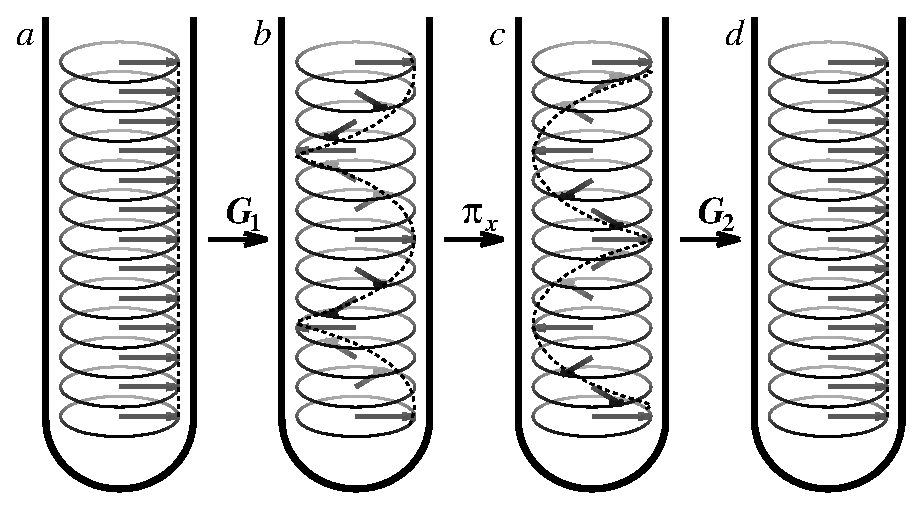
\epsfig{file=gradecho.eps,width=4in}
\end{center}
\caption[Écho de spin avec gradient]{Écho de spin avec gradient.
$a$. Aimantation transversale initiale. 
$b$. effet de la première impulsion de gradient. 
$c$. Inversion de l'aimantation.
$d$. effet de la seconde impulsion de gradient.}
\label{fig:gradecho}
\end{figure}

\section{Matrice densité et modèle vectoriel}
La présentation du modèle vectoriel pour les systèmes de spins isolés est l'objet
du chapitre \ref{chap:bloch}.

De la même manière qu'un système à un spin est caractérisé par une unique
fréquence de résonance et est classiquement décrit par un seul vecteur aimantation,
un système de deux spins faiblement couplés est caractérisé par quatre fréquences
de résonance et est décrit, dans le cadre du modèle vectoriel, par quatre vecteurs.

Les quatre états de spin $\al\al$, $\be\al$, $\al\be$ et $\be\be$ sont liés par quatre
transitions à $\pm 1$ quanta, comme indiqué sur la figure \ref{fig:diagramisj}.
Deux vecteurs aimantation seront associés aux transitions du noyau $I$
et deux au noyau $S$.
L'aimantation d'équilibre du noyau $I$ résulte de la somme des différences de populations :
\begin{equation}
\Delta P(I) = (p_{\al\al} - p_{\be\al}) + (p_{\al\be} - p_{\be\be})
\end{equation}
Le modèle vectoriel considère l'évolution des deux composantes de l'aimantation dues
aux noyaux $I$ d'une part et de des deux composantes dues aux noyaux $S$ d'autre part.
Pour chaque noyau, une composante diffère de l'autre par l'état $\al$ ou $\be$
de l'autre noyau.
La composante notée $\aimvec_{I\al}$ correspond à la paire d'états
($\al\al$, $\be\al$) liée à la transition du noyau $I$ quand le noyau $S$ 
se trouve dans l'état $\al$.
La fréquence de cette transition est $\nu_1 = \nu_I - J/2$.
La composante transversale du vecteur $\aimvec_{I\al}$ est sujette à un mouvement
de précession de fréquence $\nu_1$ dans le référentiel du laboratoire.
Le système $IS$ est décrit par l'ensemble des quatre
vecteurs $\aimvec_{I\al}$, $\aimvec_{I\be}$,
$\aimvec_{\al S}$ et $\aimvec_{\be S}$. 

La matrice densité d'un système de 2 spins évolue dans un espace de dimension 16, alors
qu'un ensemble de 4 vecteurs dans un espace physique de dimension 3 ne fait intervenir
que 12 coordonnées.
Les 4 (16 $-$ 12) coordonnées manquantes sont celles qui décrivent les 4 cohérences à
0 et $\pm$ 2 quanta du système.
Tant que l'on ne cherche pas à mettre en {\oe}uvre des expériences fondées sur des évolutions
autres que celles des populations et des cohérences d'ordre $\pm 1$,
le modèle vectoriel est susceptible de fournir une
interprétation graphique correcte des observations.

Du point de vue du formalisme des opérateurs, les trois coordonnées du
vecteur $\aimvec_{I\al}$ sont fournies par les coefficients multiplicatifs
des opérateurs $I_xS_{\al}$, $I_yS_{\al}$ et $I_zS_{\al}$, la matrice densité
étant exprimée dans ce qui pourrait être une base
\{
$I_xS_{\al}$, $I_yS_{\al}$, $I_zS_{\al}$,
$I_xS_{\be}$, $I_yS_{\be}$, $I_zS_{\be}$,
$I_{\al}S_x$, $I_{\al}S_y$, $I_{\al}S_z$,
$I_{\be}S_x$, $I_{\be}S_y$, $I_{\be}S_z$
\}
du sous-espace des états susceptibles d'être décrits par le formalisme vectoriel.
Ce n'est pas une base car
\begin{eqnarray}
\label{eqn:izsza}
2I_zS_z & = & I_z(S_{\al}-S_{\be}) = I_zS_{\al} - I_zS_{\be} \\
\label{eqn:izszb}
2I_zS_z & = & (I_{\al}-I_{\be})S_z = I_{\al}S_z - I_{\be}S_z
\end{eqnarray}
et en sachant qu'un même état ne peut être décrit de deux manières différentes
comme combinaisons linéaires des mêmes états de base.
Toutefois, cet ensemble de 12 éléments contient 8 états d'ordre de cohérence $\pm 1$
qui constituent une base.
Le modèle vectoriel est donc particulièrement adapté au suivi de l'évolution
de l'aimantation transversale.
L'extension aux opérateurs de population est néanmoins acceptable,
sous réserve de ne pas être trop sourcilleux sur la rigueur mathématique.

L'état initial du système, en omettant la partie proportionnelle
à la matrice identité, s'écrit :
\begin{eqnarray}
\sigma_0 & = & \Delta P(I)/2 \cdot I_z + \Delta P(S)/2 \cdot S_z\\
& = & \frac{1}{2}\left(
\Delta P(I)(I_zS_{\al} + I_zS_{\be}) 
+ \Delta P(S)(I_{\al}S_z + I_{\be}S_z) 
\right)
\end{eqnarray}
ce qui correspond graphiquement à la figure \ref{fig:vectisinit}
où la superposition des paires de vecteurs identiques est remplacée
par une flèche double.
La partie gauche de la figure se rapporte au noyau $I$ et
les annotations $\al$ et $\be$ décrivent l'état de spin du noyau $S$.

\begin{figure}[hbt]
\begin{center}
\begin{pspicture}(-3,-2)(3,3)
\SpecialCoor
\psline{->}(0.5;150)(2.5;-30)
\psline{->}(0.5;270)(2.5;90)
\psline{->}(0.5;30)(2.5;210)
\psline[linewidth=0.06,doubleline=true,doublesep=0.05]{->}(0,0)(2;90)
\uput[210](2.5;210){$X$}
\uput[-30](2.5;-30){$Y$}
\uput[90](2.5;90){$Z$}
\rput(-0.5,0){$O$}
\rput(2;90){\rput(-0.25,0){$\alpha$}\rput(0.25,0){$\beta$}}
\rput(0,-1.75){I}
\end{pspicture}
\begin{pspicture}(-3,-2)(3,3)
\SpecialCoor
\psline{->}(0.5;150)(2.5;-30)
\psline{->}(0.5;270)(2.5;90)
\psline{->}(0.5;30)(2.5;210)
\psline[linewidth=0.06,doubleline=true,doublesep=0.05]{->}(0,0)(1;90)
\uput[210](2.5;210){$X$}
\uput[-30](2.5;-30){$Y$}
\uput[90](2.5;90){$Z$}
\rput(-0.5,0){$O$}
\rput(1;90){\rput(-0.25,0){$\alpha$}\rput(0.25,0){$\beta$}}
\rput(0,-1.75){S}
\end{pspicture}

\caption{\label{fig:vectisinit}
\small Représentation vectorielle de l'état initial d'un système $IS$}
\end{center}
\end{figure}

Une impulsion de RF $\pi/2_y$ appliquée à la fréquence de $I$ amène l'aimantation
sur l'axe $OX$ du référentiel tournant lié à $I$.
En d'autres termes :
\begin{equation}
I_zS_{\al} \flham{\pi/2_y} I_xS_{\al}
\qetq
I_zS_{\be} \flham{\pi/2_y} I_xS_{\be}
\end{equation}

Les vecteurs $\aimvec_{I\al}$ et $\aimvec_{I\be}$, superposés sur l'axe $OX$
juste après l'impulsion, vont ensuite évoluer à leur pulsation de précession propres
$\Omega_{I\alpha} = \omsi - \pi J$ et 
$\Omega_{I\beta} = \omsi + \pi J$ dans le référentiel tournant,
comme sur la figure \ref{fig:vectisevol} limitée à la représentation
du plan transversal $XOY$.
Après un temps $t$ dévolution libre du système sous l'action de 
l'hamiltonien $H$, $\aimvec_{I\alpha}$ et $\aimvec_{I\beta}$ tournent
respectivement des angles $\theta_{\alpha} = \Omega_{I\alpha} t$ et
$\theta_{\beta} = \Omega_{I\beta} t$.
L'angle entre les deux vecteurs est $2\pi J t$.

\begin{figure}[hbt]
\begin{center}
\begin{pspicture}(-6,-2)(6,2)
\SpecialCoor
\rput(-4,0){
\pscircle(0,0){1.5}
\psline{->}(2;180)(2;0)
\psline{->}(2;-90)(2;90)
\uput[0](2;0){$X$}
\uput[90](2;90){$Y$}
\psline[linewidth=0.06,doubleline=true,doublesep=0.05]{->}(0,0)(1.5;0)
\uput[0](1.5;0){\rput(0,-0.25){$\alpha$}\rput(0,0.25){$\beta$}}
}
\rput(4,0){
\pscircle(0,0){1.5}
\psline{->}(2;180)(2;0)
\psline{->}(2;-90)(2;90)
\uput[0](2;0){$X$}
\uput[90](2;90){$Y$}
\psline[linewidth=0.06]{->}(0,0)(1.5;150)
\psline[linewidth=0.06]{->}(0,0)(1.5;80)
\uput[80](1.5;80){$\alpha$}
\uput[150](1.5;150){$\beta$}
\psarc[arcsepB=0.06,linewidth=0.02]{->}(0,0){0.9}{0}{80}
\psarc[arcsepB=0.06,linewidth=0.02]{->}(0,0){1.0}{0}{150}
\uput[220](1.1;40){$\theta_{\alpha}$}
\uput[120](0.8;120){$\theta_{\beta}$}
}
\psline[linewidth=0.04]{->}(-0.75,0)(0.75,0)
\rput(0,0.25){$Ht$}
\end{pspicture}
\caption{\label{fig:vectisevol}
\small Evolution de l'aimantation transversale du noyau $I$ d'un syst\`eme $IS$}
\end{center}
\end{figure}

La détection des deux composantes de l'aimantation de $I$ conduit après TF 
à un doublet de lorentziennes en phase
de fréquences séparées de la constante de couplage $J$ et centrées sur $\nu_I$.
Le même raisonnement peut être effectué indépendemment (système $IS$ hétéronucléaire)
ou simultanément (système $IS$ homonucléaire) pour le noyau S.

Le modèle vectoriel aide à visualiser
simplement l'action d'un écho de spin de durée $2T$ sur l'aimantation transversale 
du noyau $I$ d'un système $IS$ hétéronucléaire,
et ceci dans les trois situations possibles (figure \ref{fig:vectecho}) :

\begin{figure}[hbt]
\begin{center}
\begin{pspicture}(-6,-3)(6,3)
\SpecialCoor
\psset{labelsep=2pt}
\rput(-3.75,0){
\rput(-1.75,0){
\pscircle(0,0){0.75}
\psline[linewidth=0.04,doubleline=true,doublesep=0.03]{->}(0,0)(0.75;0)
\uput[-10](0.75;-10){$\alpha$}
\uput[10](0.75;10){$\beta$}
}
\rput(1.75,0){
\pscircle(0,0){0.75}
\psline[linewidth=0.04]{->}(0,0)(0.75;50)
\uput[50](0.75;50){$\alpha$}
\psline[linewidth=0.04]{->}(0,0)(0.75;70)
\uput[70](0.75;70){$\beta$}
}
\psline[linewidth=0.03]{->}(-0.5,0)(0.5,0)
\rput(0,0.25){$HT$}
}
\rput(-0.75,0){
\psline[linewidth=0.03]{->}(0,0)(1.5,0)
\psline[linewidth=0.03]{->}(0.25,0)(0.5,2.25)(1.5,2.25)
\psline[linewidth=0.03]{->}(0.25,0)(0.5,-2.25)(1.5,-2.25)
\rput(1,2.5){$\pi_x(I)$}
\rput(1,0.25){$\pi_x(S)$}
\rput(1,-2){$\pi_x(I)$}
\rput(1,-2.5){$\pi_x(S)$}
}
\rput(3.75,0){
\rput(0,2.25){
\rput(-1.75,0){
\pscircle(0,0){0.75}
\psline[linewidth=0.04]{->}(0,0)(0.75;-50)
\uput[-50](0.75;-50){$\alpha$}
\psline[linewidth=0.04]{->}(0,0)(0.75;-70)
\uput[-70](0.75;-70){$\beta$}
}
\rput(1.75,0){
\pscircle(0,0){0.75}
\psline[linewidth=0.04,doubleline=true,doublesep=0.03]{->}(0,0)(0.75;0)
\uput[-10](0.75;-10){$\alpha$}
\uput[10](0.75;10){$\beta$}
}
\psline[linewidth=0.03]{->}(-0.5,0)(0.5,0)
\rput(0,0.25){$HT$}
}
\rput(0,0){
\rput(-1.75,0){
\pscircle(0,0){0.75}
\psline[linewidth=0.04]{->}(0,0)(0.75;50)
\uput[50](0.75;50){$\beta$}
\psline[linewidth=0.04]{->}(0,0)(0.75;70)
\uput[70](0.75;70){$\alpha$}
}
\rput(1.75,0){
\pscircle(0,0){0.75}
\psline[linewidth=0.04,doubleline=true,doublesep=0.03]{->}(0,0)(0.75;120)
\uput[110](0.75;110){$\beta$}
\uput[130](0.75;130){$\alpha$}
}
\psline[linewidth=0.03]{->}(-0.5,0)(0.5,0)
\rput(0,0.25){$HT$}
}
\rput(0,-2.25){
\rput(-1.75,0){
\pscircle(0,0){0.75}
\psline[linewidth=0.04]{->}(0,0)(0.75;-50)
\uput[-50](0.75;-50){$\beta$}
\psline[linewidth=0.04]{->}(0,0)(0.75;-70)
\uput[-70](0.75;-70){$\alpha$}
}
\rput(1.75,0){
\pscircle(0,0){0.75}
\psline[linewidth=0.04]{->}(0,0)(0.75;20)
\uput[20](0.75;20){$\beta$}
\psline[linewidth=0.04]{->}(0,0)(0.75;-20)
\uput[-20](0.75;-20){$\alpha$}
}
\psline[linewidth=0.03]{->}(-0.5,0)(0.5,0)
\rput(0,0.25){$HT$}
}
}
\end{pspicture}
\caption{\label{fig:vectecho}
\small Évolution de l'aimantation transversale du noyau $I$ d'un système $IS$ pendant un
écho de spin.}
\end{center}
\end{figure}

\begin{enumerate}
\item Seul $I$ subit une impulsion RF $\pi_x$. Pendant la deuxième partie de l'écho
chaque composante décrit exactement le même angle que pendant la première partie.
Elle se retrouvent à leur emplacement initial quel que soit $\omsi$ et $J$.
Les effets du couplage et de l'offset de $I$ sont refocalisés.
\item Seul $S$ subit une impulsion RF $\pi_x$. L'impulsion sur $S$ permute les
"étiquettes" $\al$ et $\be$ :
\begin{equation}
S_{\al} \flham{\pi_x(S)} S_{\be}
\qetq
S_{\be} \flham{\pi_x(S)} S_{\al}
\end{equation}
avec pour conséquence que chaque composante à tourné à la pulsation
$\omsi + \pi J$ pendant $T$ et $\omsi - \pi J$ aussi pendant $T$.
Les composantes se superposent au temps $2T$ comme si elles avaient tourné
à la pulsation $\omsi$.
L'effet du couplage est refocalisé.
\item $I$ et $S$ subissent une impulsion RF $\pi_x$.
Le vecteur $\aimvec_{I\al}$ a tourné à la pulsation $\omsi - \pi J$ pendant
la première période, est devenu $\aimvec_{I\be}$ par action de l'impulsion
$\pi_x(S)$ et a tourné à la pulsation $\omsi + \pi J$ pendant
la seconde période. 
Tout se passe comme si seul le couplage avait agit pendant $2T$.
L'effet de l'offset de $I$ (et de $S$, par symétrie) est refocalisé.
\end{enumerate}

Le lecteur pourra constater qu'utiliser une impulsion $\pi_y$ transforme les
vecteurs finaux en leur opposé, en plein accord avec la description
de l'écho de spin utilisant la matrice densité.
Ce tableau du modèle vectoriel sera complété lors de l'étude du transfert
d'aimantation cohérent.

L'extension du modèle à un système $ISL$ faiblement couplé fait apparaître
pour chaque noyau quatre composantes.
Ainsi, celles du noyau$ $I seront notées $\aimvec_{I\al\al}$,
$\aimvec_{I\be\al}$, $\aimvec_{I\al\be}$ et $\aimvec_{\be\be}$.
Les principes exposés aux paragraphes précédents s'appliquent
de manière immédiate.
